\documentclass[10pt]{report}

\usepackage{stan-talks}

\begin{document}
\sf%
\vspace*{-12pt}
%
\noindent 
\spc{\Huge\bfseries \color{MidnightBlue}{Stan under the hood}}
\\[16pt]
\noindent 
\spc{\Large\bfseries \color{MidnightBlue}{Bob Carpenter}}
\\[6pt]
\spc{\large Center for Computational Mathematics}
\\
\spc{\large Flatiron Institute}
\\[12pt]
\spc{Stan 2.36 (March 2025)
\\
\spc{\bfseries \url{https://mc-stan.org}}}
\hfill
\vfill
\hfill

\includegraphics[height=0.25in]{img/fi-logo.png}
\qquad 

\includegraphics[height=0.5in]{img/new-logo.png}

\sld{Who is Stan?}
%
\begin{itemize}
\item Stan is named in honor of \myemph{Stanislaw Ulam} (1909--1984)
\item Co-inventor of the \myemph{Monte Carlo method}
\item[]
\vspace*{4pt}
  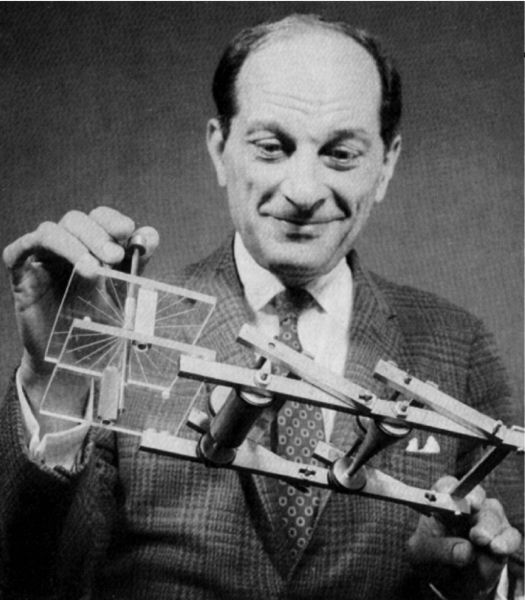
\includegraphics[width=0.2\textwidth]{img/ulam-fermiac.jpg}
\\[2pt] \footnotesize Ulam holding the Fermiac, Enrico Fermi's physical Monte Carlo simulator
  for random neutron diffusion; \hfill
\\[4pt]
{\tiny \mbox{ } \hfill image from G.~C.~Geisler (2000) Los Alamos report LA-UR-2532}
\end{itemize}

\sld{What is Stan?}
%
\begin{itemize}
\item Stan is an \myemph{imperative probabilistic programming language}
  \begin{subitemize}
  \item  cf., BUGS: declarative; \ Church: functional; \ Figaro: OO
  \end{subitemize}
\item Stan \myemph{program}: defines a probability model
  \begin{subitemize}
  \item declares data and (constrained) parameter variables
  \item defines log posterior (or penalized likelihood)
  \item defines posterior predictive quantities
  \end{subitemize}
\item Stan \myemph{inference}: fits model to data \& makes predictions
  \begin{subitemize}
  \item MCMC for full Bayesian inference (NUTS)
  \item VB for approximate Bayesian inference (ADVI, Pathfinder)
  \item Laplace approximation and MLE (L-BFGS)
  \end{subitemize}
\end{itemize}


\sld{Why Choose Stan?}
%
\begin{itemize}
\item \myemph{Expressive}
\begin{subitemize}
\item Stan is a domain-specific, differentiable imperative programming language for coding probability models.
\end{subitemize}
\item \myemph{Robust}
\begin{subitemize}
\item usually works; signals when it doesn't
\end{subitemize}
\item \myemph{Efficient}
\begin{subitemize}
\item effective sample size / time remains state-of-the-art (on CPU)
\item multi-core and GPU support (not competitive with JAX)
\end{subitemize}
\item Ongoing \myemph{open source} development.
\item \myemph{Not-so Secret Sauce}: documentation and friendly \myemph{Stan community}!
\end{itemize}


\sld{It's 2010, why build Stan?  \hfill \large (1/6)}
%
\begin{itemize}
\item {\slshape\bfseries Goal}: Andrew Gelman hired me and Matt Hoffman to find a way to robustly describe and models in his and Jennifer Hill's multilevel regression book.
\end{itemize}
%
\vspace*{2pt}
\begin{itemize}
\item {\slshape Problem}: Gibbs and Metropolis too slow (diffusive)
\item {\slshape Solution}: Hamiltonian Monte Carlo (flow)
%
\vspace*{8pt}
\item {\slshape Problem}:  Interpreters slow and unscalable
\item {\slshape Solution}: Compile to C++ (my own background was in NLP and PL theory)
%
\vspace*{8pt}
\item {\slshape Problem}:  Need gradients of log posterior for HMC
\item {\slshape Solution}: Reverse-mode automatic differentiation (fortuitous blog response)
\end{itemize}


\sld{Why Stan? \hfill \large (2/6)}
%
\begin{itemize}
\item {\slshape Problem}:  Existing autodiff slow and limited (before PyTorch/TensorFlow)
\item {\slshape Solution}: Engineer our own autodiff.
%
\vspace*{8pt}
\item {\slshape Problem}:  Autodiff requires functions templated on
  all arguments.
\item {\slshape Solution}: Our own density and special functions library, Eigen linear algebra, Boost foundation (bulk of our dev cost)
%
\vspace*{8pt}
\item {\slshape Problem}:  Need unconstrained parameters for HMC.
\item {\slshape Solution}: Variable transforms w. Jacobian determinants behind the scenes.
%
\end{itemize}


\sld{Why Stan? \hfill \large (3/6)}
%
\begin{itemize}
\item {\slshape Problem}:  Need ease of use of BUGS.
\item {\slshape Solution}: Compile a domain-specific language.
%
\vspace*{8pt}
\item {\slshape Problem}:  Pure directed graphical language inflexible.
\item {\slshape Solution}: Imperative probabilistic/differentiable programming.
  language.
\vspace*{8pt}
\item {\slshape Problem}:  Need to tune parameters for HMC.
\item {\slshape Solution}: Tune step size and estimate mass matrix
  during warmup;  on-the-fly number of steps (NUTS).
%
\end{itemize}


\sld{Why Stan? \hfill \large (4/6)}
%
\begin{itemize}
%
\vspace*{4pt}
\item {\slshape Problem}:  Efficient up-to-proportion density calcs.
\item {\slshape Solution}: Density template metaprogramming.
%
\vspace*{4pt}
\item {\slshape Problem}:  Limited error checking, recovery.
\item {\slshape Solution}: Static model typing, informative exceptions.
%
\vspace*{4pt}
\item {\slshape Problem}:  Poor numerical stability.
\item {\slshape Solutions}:
{
Taylor expansions, e.g., {\small \code{log1p()}}
\\[2pt]
compound functions, e.g., {\small \code{log\_sum\_exp()}, \
\code{BernoulliLogit()}}
\\[2pt]
limits at boundaries, e.g., {\small \code{multiply\_log()}}
}
%
\end{itemize}


\sld{Why Stan? \hfill \large (5/6)}
%
\begin{itemize}
\item {\slshape Problem}:  Nobody knows everything.
\item {\slshape Solution}: Expand project team with specialists in stats and software.
\vspace*{8pt}
\item {\slshape Problem}:  Expanding code and project team!
\item {\slshape Solution}: GitHub: branch, pull
  request, code review.
\item {\slshape Solution}: Jenkins: continuous integration.
\item {\slshape Solution}: Ongoing refactoring and code simplification.
%
\end{itemize}


\sld{Why Stan? \hfill \large (6/6)}
%
\begin{itemize}
\item {\slshape Problem}:  Heterogeneous user base.
\item {\slshape Solution}: More interfaces (R, Python, MATLAB, Julia).
\item {\slshape Solution}:  Domain-specific examples, tutorials.
\vspace*{8pt}
\item {\slshape Problem}:  Restrictive licensing limits use.
\item {\slshape Solution}: Code and doc open source (BSD, CC-BY)
\end{itemize}

\sld{\Large What Stan Computes \hfill \large (1/2)}
%
\begin{itemize}
%
\item \myemph{MCMC draws} from posterior $p(\theta \mid y)$:
\[
\theta^{(1)}, \ldots, \theta^{(M)} \sim p(\theta \mid y).
\]
\item Posterior \myemph{parameter estimates}
\[
\hat{\theta}
\ = \
\mathbb{E}[\theta \mid y]
\ = \
\int \theta \cdot p(\theta \mid y) \, \mathrm{d}\theta
\ \approx \
\frac{1}{M} \sum_{m=1}^M \theta^{(m)}
\]
%
\item Posterior \myemph{parameter variance estimates}
\[
\mathrm{var}[\theta \mid y]
\ = \
\mathbb{E}[(\theta - \hat{\theta})^2 \mid y]
\ = \
\int (\theta - \hat{\theta})^2 \cdot p(\theta \mid y) \, \mathrm{d}\theta
\ \approx \
\frac{1}{M} \sum_{m=1}^M (\theta^{(m)} - \hat{\theta})^2
\]
\end{itemize}


\sld{\Large What Stan Computes \hfill \large (2/2)}
%
\begin{itemize}
\item Posterior \myemph{event probabilities} for event $A \subseteq \Theta$
\[
\mbox{Pr}[\textrm{I}_A(\theta) \mid y]
\ = \
\mathbb{E}[\textrm{I}_A(\theta) \mid y]
\ = \
\int \textrm{I}_A(\theta) \cdot p(\theta \mid y)
\, \mathrm{d}\theta
\ \approx \
\frac{1}{M} \sum_{m=1}^M \mathrm{I}_A(\theta^{(m)}).
\]
%
\item Posterior \myemph{predictions} for new data $\tilde{y}$
\[
p(\tilde{y} \mid y)
 =
\mathbb{E}[p(\tilde{y} \mid \theta) \mid y]
\ = \
\int p(\tilde{y} \mid \theta) \cdot p(\theta \mid y) \, \mathrm{d}\theta
\ \approx \
\frac{1}{M} \sum_{m=1}^M p\left( \tilde{y} \mid \theta^{(m)} \right)
\]
%
\item Posterior \myemph{quantiles} (e.g., \myemph{intervals} and \myemph{median})
\[
\mathrm{quantile}(\theta, \alpha)
\ = \
\mathrm{sort\_ascending}(\theta^{(1)}, \ldots, \theta^{(M)})
\left[ \, \lceil \alpha \times M \rceil \, \right]
\]
\end{itemize}

\sld{Laplace's birth rate by sex study}
\begin{itemize}
\item \myemph{Laplace}'s data on live births in Paris from 1745--1770:
\vspace*{-4pt}
\begin{center}\small
\begin{tabular}{c|c}
{\slshape sex} & {\slshape live births}
\\ \hline
female & 241\,945
\\
male & 251\,527
\end{tabular}
\end{center}
\item \myemph{Question 1} (Estimation)
\\
What is the birth rate of boys vs. girls?

\item \myemph{Question 2} (Event Probability)
\\
Is a boy more likely to be born than a girl?
%
\item Bayes (1763) set up the ``Bayesian'' model.
\item Laplace (1781, 1786) solved for the posterior analytically.
\end{itemize}
  
\sld{Laplace's model in Stan}
%
\begin{stancode}
transformed data {
  int male = 251527;
  int female = 241945;
}
parameters {
  real<lower=0, upper=1> theta;
}
model {
  male ~ binomial(male + female, theta);
}
generated quantities {
  int<lower=0, upper=1> theta_gt_half = (theta > 0.5);
}
\end{stancode}

\sld{And the Answer is...}
%
\begin{codein}
> fit <- stan("laplace.stan", iter=100000);
> print(fit, probs=c(0.005, 0.995), digits=3)
\end{codein}
\begin{codeout}
                    mean   0.5%  99.5%
theta               0.51  0.508  0.512
theta_gt_half       1.00  1.000  1.000 (*)
\end{codeout}
%
\begin{itemize}
\item Q1: $\theta$ is 99\% certain to lie in $(0.508, 0.512)$
%
\item Q2:  Laplace ``morally certain'' boys more prevalent
  \vfill
\item (*) Stan reports 100\% MCMC estimate because true probability is $1 - 10^{-42}$!
\end{itemize}

\sld{Linear Regression with Prediction}
%
\begin{stancode}
data {
  int<lower=0> K;   int<lower=0> N;    int<lower=0> N_tilde; 
  matrix[N, K] x;   vector[N] y;       matrix[N_tilde, K] x_tilde;
}
parameters {
  vector[K] beta;   real<lower=0> sigma;
}
model {
  y ~ normal(x * beta, sigma);                           // likelihood
  beta ~ normal(0, 1);          sigma ~ exponential(1);  // prior
}
generated quantities {
  vector[N_tilde] y_tilde = normal_rng(x_tilde * beta, sigma);  // predictive
}
\end{stancode}

\sld{Lynxes and Hares}
%
\begin{center}
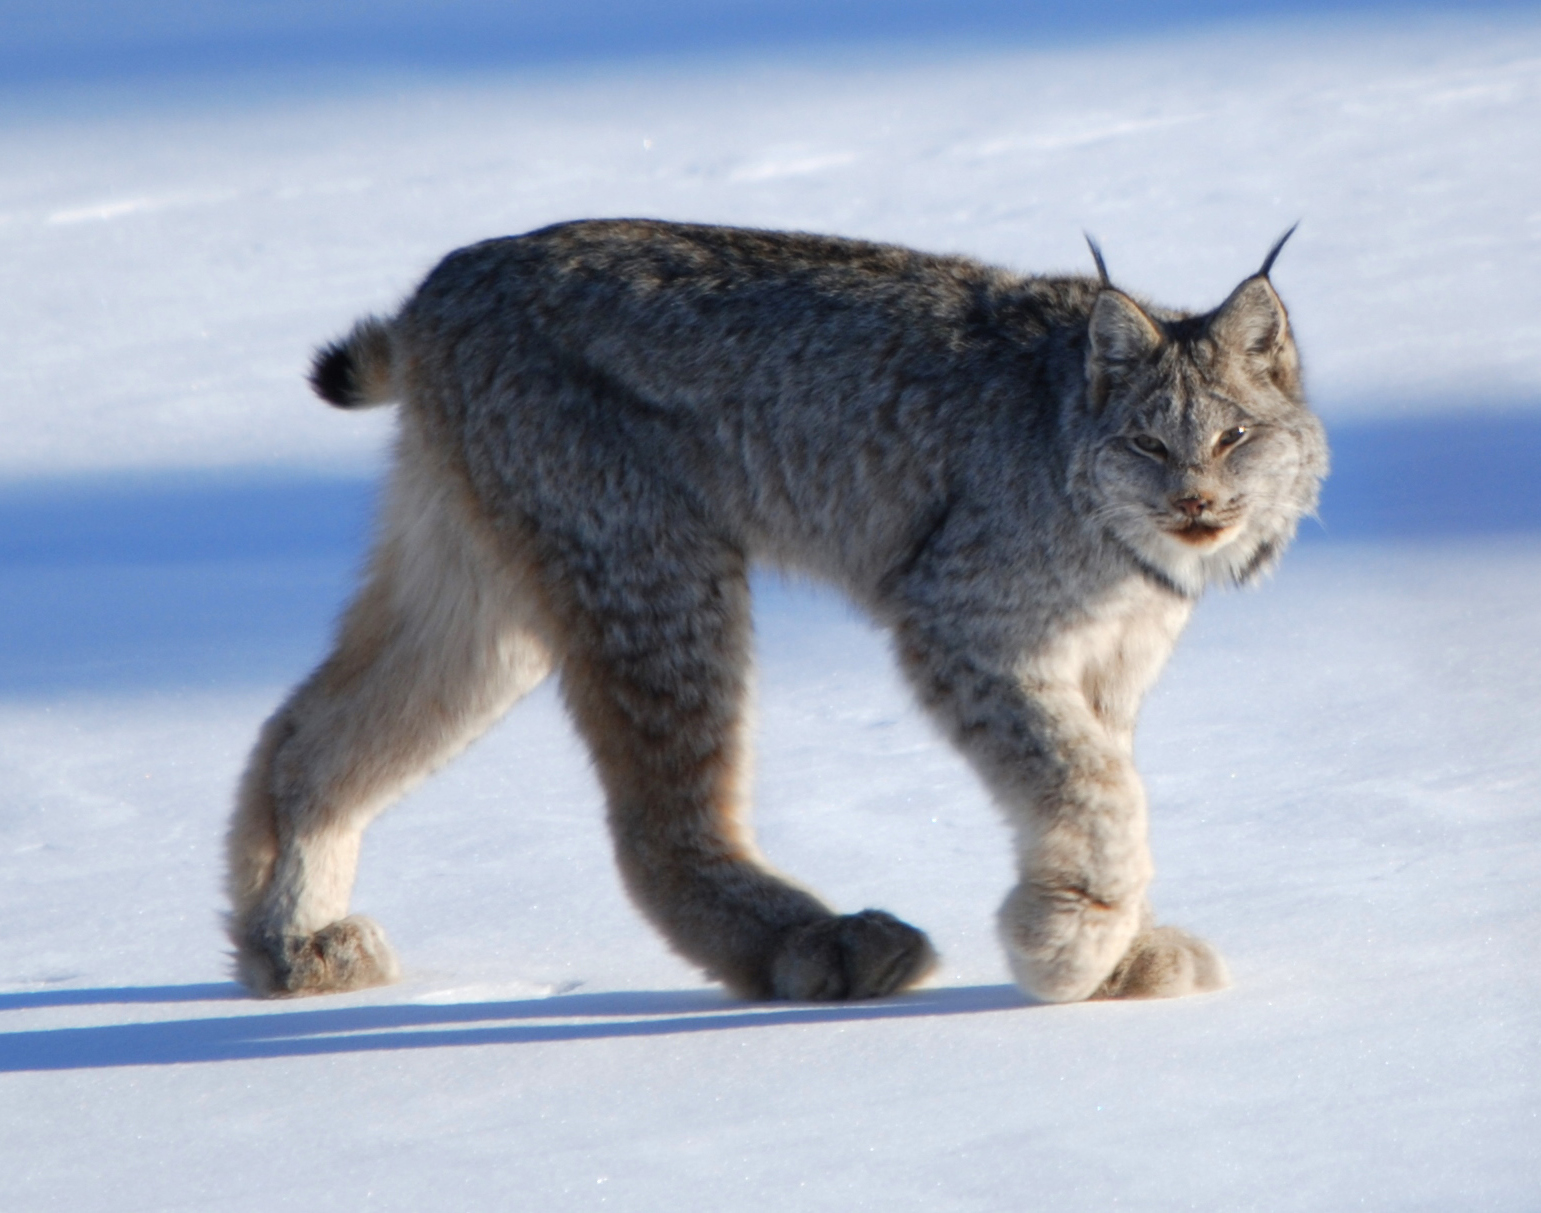
\includegraphics[height=1in]{img/lynx.jpg}
\hspace*{0.25in}
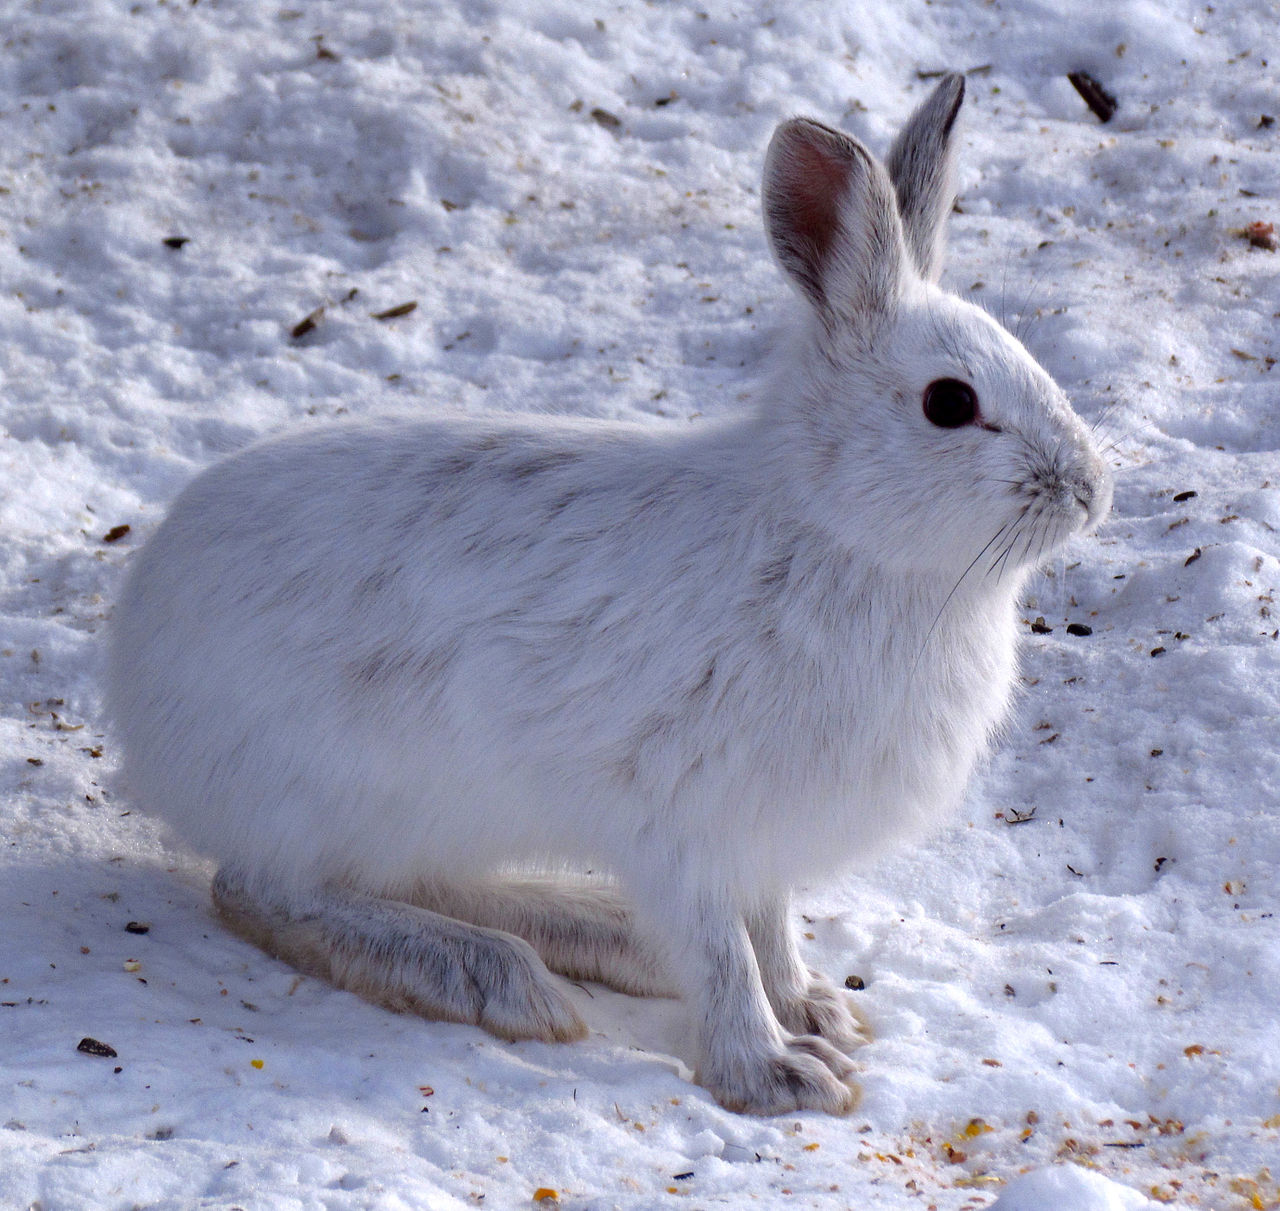
\includegraphics[height=1in]{img/hare.jpg}
\end{center}
\begin{itemize}
\item \myemph{Snowshoe hare} (prey): herbivorous cousin of rabbits
\item \myemph{Canadian lynx} (predator): feline eating primarily hares
\end{itemize}
\vfill
{\tiny
\mbox{ } \hfill
Lynx image copyright 2009, Keith Williams, CC-BY 2.0.
\\[-2pt]
\mbox{ } \hfill
Hare image copyright 2013 D. Gordon E. Robonson, CC-BY SA 2.0}


\sld{Hudson Bay Co. Pelts, 1900--20}
%
\vspace*{6pt}
\begin{center}
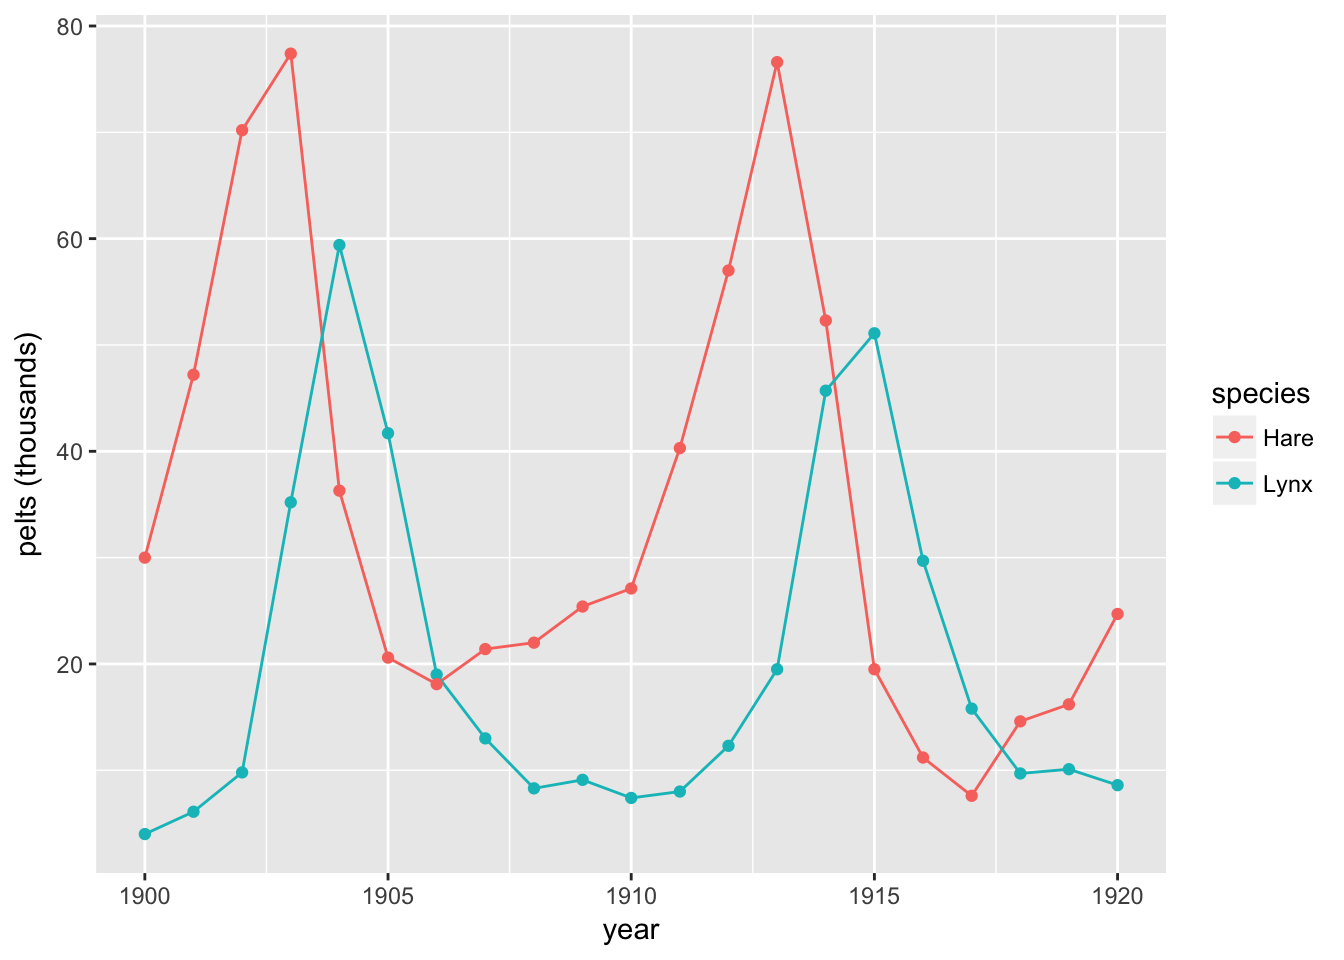
\includegraphics[width=0.6\textwidth]{img/hare-lynx-pelts-1.png}
\end{center}

\sld{Pelts, Phase Space}
%
\vspace*{6pt}
\begin{center}
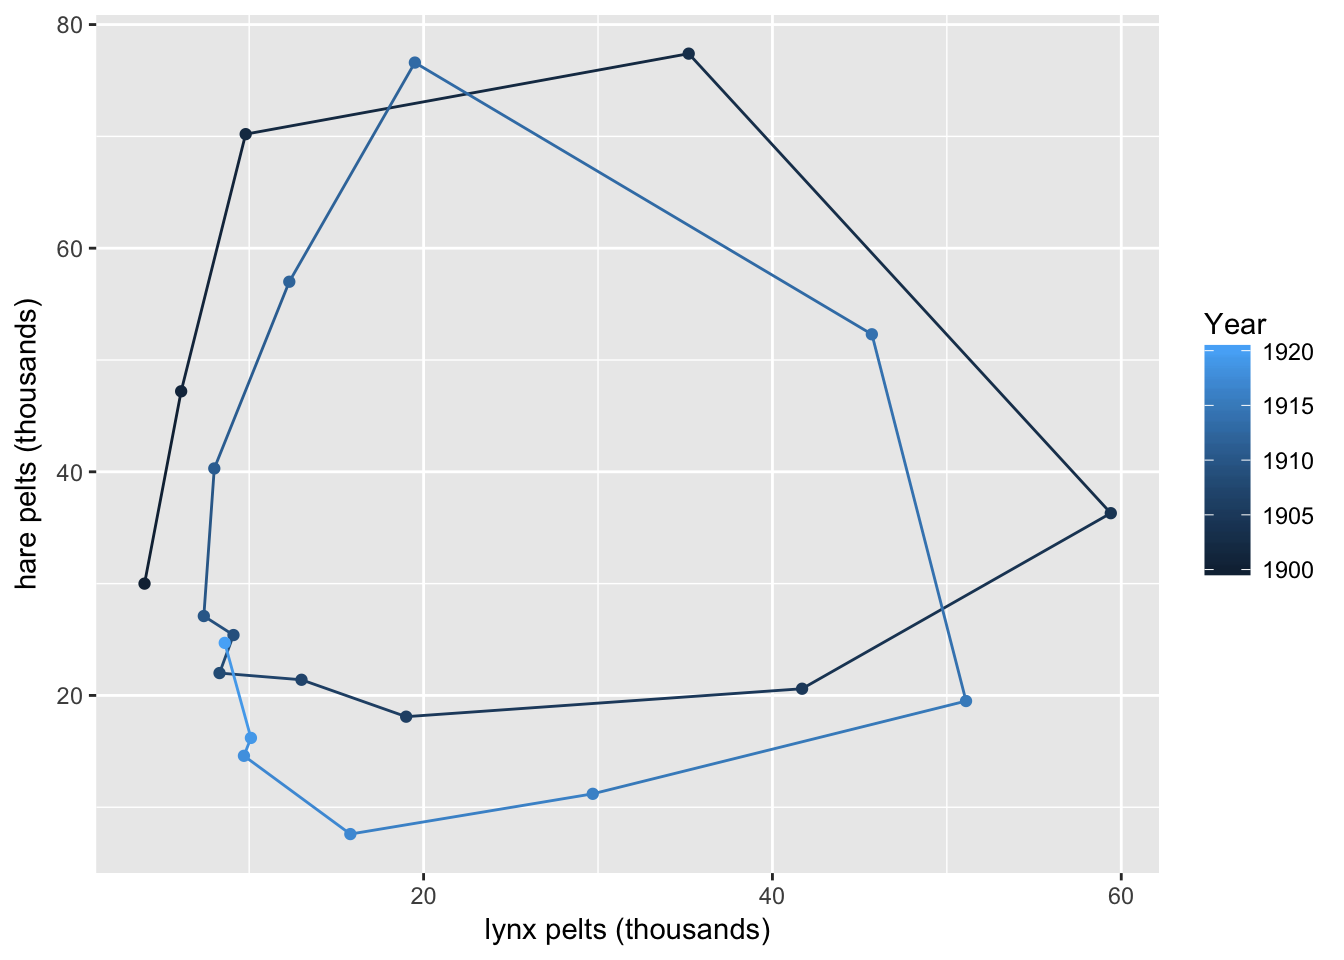
\includegraphics[width=0.6\textwidth]{img/hare-lynx-pelts-2.png}
\end{center}

\sld{Volterra's (1927) Model}
%

\begin{minipage}[t]{0.5\textwidth}
\vspace*{-0.75in}
  \begin{subitemize}
\item population: $u(t)$ \myemph{prey}, \ $v(t)$ \myemph{predator}
%
\begin{eqnarray*}
\frac{\mathrm{d}}{\mathrm{d}t} u
& = &  (\alpha - \beta v) u
\\[6pt]
\frac{\mathrm{d}}{\mathrm{d}t} v
& = &  (-\gamma + \delta \, u) \, v
\end{eqnarray*}
%
\begin{subsubitemize}
\item $\alpha$: prey growth, intrinsic
\item $\beta$: prey shrinkage due to predation
\item $\gamma$: predator shrinkage, intrinsic
\item $\delta$: predator growth from predation
\end{subsubitemize}
\vspace*{-8pt}
\item \footnotesize dynamics lead to \myemph{oscillation} as observed
\end{subitemize}
\end{minipage}
%
\hfill
%
\begin{minipage}[t]{0.20\textwidth}
\mbox{ }
\vspace*{0.5in}
\mbox{ } \hfill
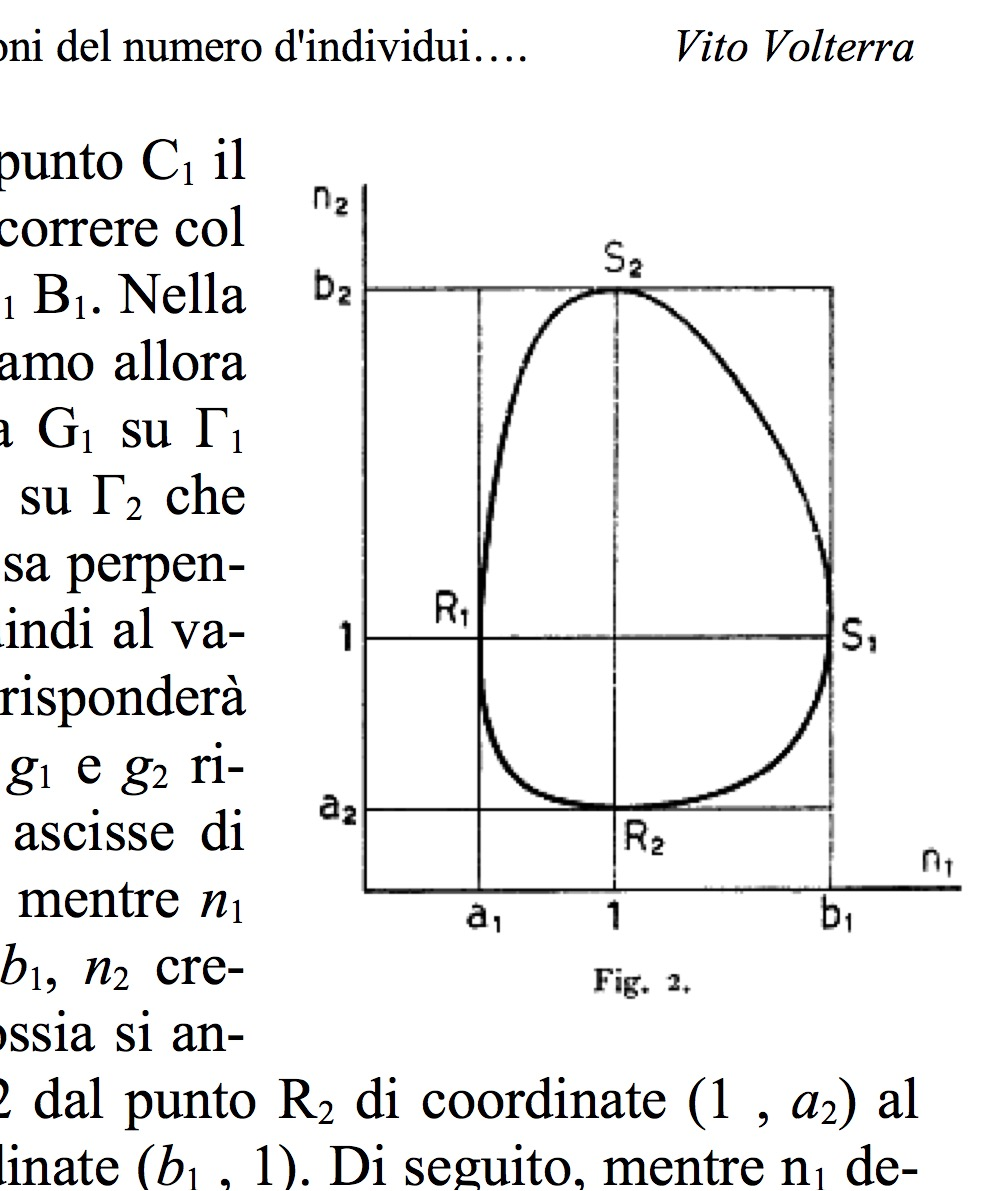
\includegraphics[width=0.7\textwidth]{img/volterra-orbit.jpg}
\\[-8pt]
\mbox{ }
\hfill
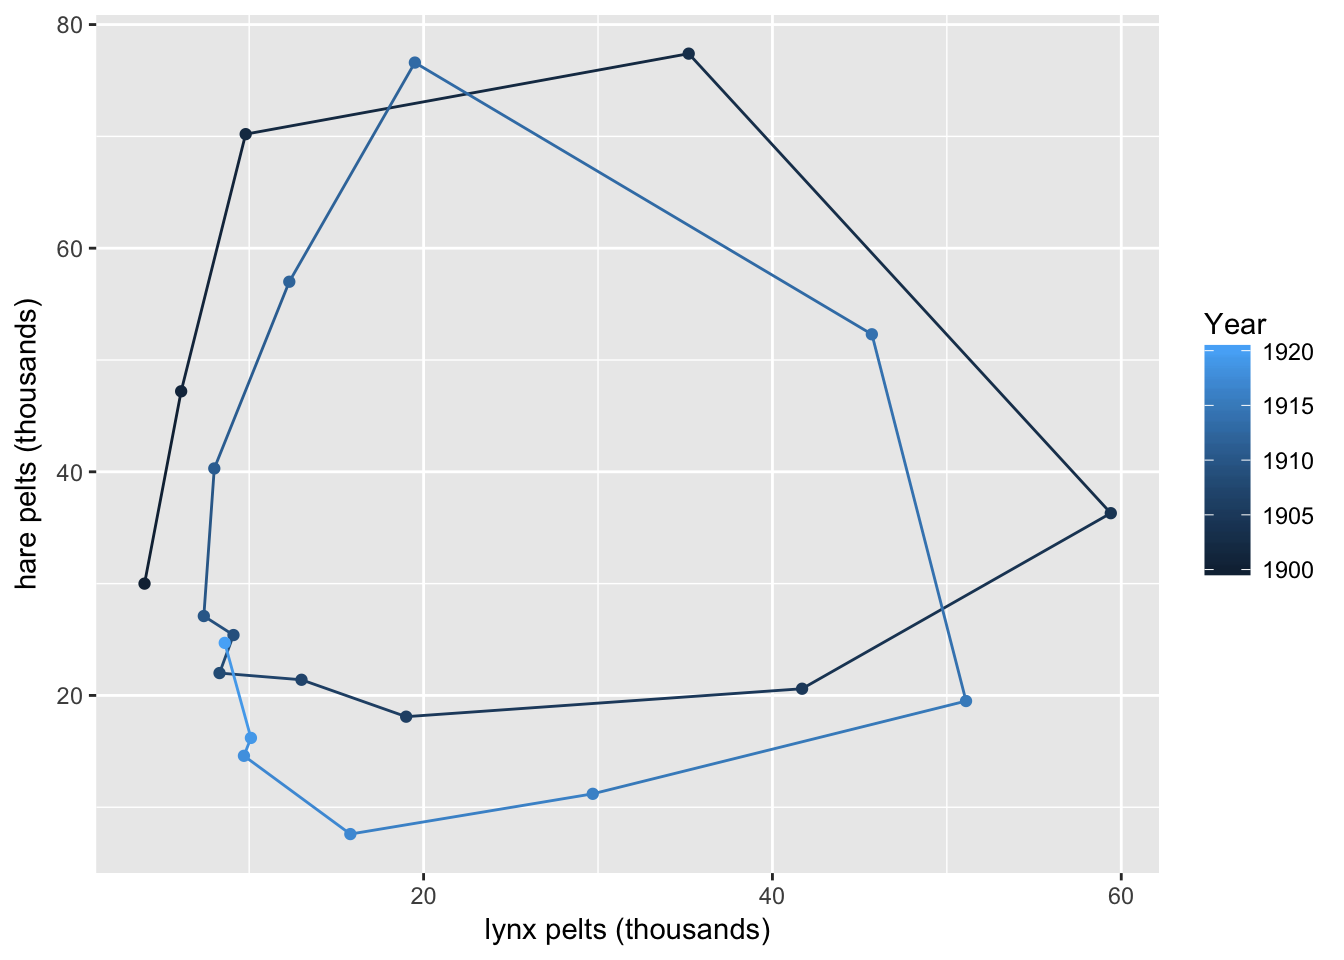
\includegraphics[width=0.7\textwidth]{img/hare-lynx-pelts-2.png}
\end{minipage}
\vfill
\hfill
{\tiny
Volterra, V., 1927. {\slshape Variazioni
e fluttuazioni del numero d'individui in specie animali
conviventi}. C.~Ferrari.
}



\sld{\Large Lotka-Volterra in Stan (dynamics)}
%
\vspace*{-2pt}
{\footnotesize
\begin{stancode}
  real[] dz_dt(data real t,       // time (unused)
               real[] z,          // system state
               real[] theta,      // parameters
               data real[] x_r,   // real data (unused)
               data int[] x_i) {  // integer data (unused)
    real u = z[1];            real v = z[2];

    real alpha = theta[1];    real beta = theta[2];
    real gamma = theta[3];    real delta = theta[4];

    real du_dt = (alpha - beta * v) * u;
    real dv_dt = (-gamma + delta * u) * v;
    return { du_dt, dv_dt };
  }
\end{stancode}
}

\sld{Data-Generating Model}
%
\vspace*{-2pt}
\begin{itemize}
\item \myemph{Known} variables are observed
\begin{subitemize}
\item  $y_{n,k}$: pelts for species $k$ at times $t_n$ for $n \in 0:N$
\end{subitemize}
\item \myemph{Unknown} variables must be inferred (\myemph{inverse problem})
\begin{subitemize}
\item initial state: $z^{\mathrm{init}}_k$: initial population for $k$
\item subsequent states $z_{n,k}$: population $k$ at time $t_n$
\item parameters $\alpha, \beta, \gamma, \delta, \sigma > 0$
\end{subitemize}
\item \myemph{Likelihood} assumes errors are proportional (not additive)
\vspace*{-8pt}
\[
y_{n, k} \sim \mathsf{LogNormal}(\hat{z}_{n,k}, \sigma_k),
\]
\vspace*{-4pt}%
{\small where $\hat{z}_n$ is \myemph{solution} at $t_n$ to L-V diff eqs for initial
$z^{\mathrm{init}}$}
\\[-3pt]
\vfill
{\small equivalently: \ $\log y_{n,k} = \log \hat{z}_{n,k} + \epsilon_{n,k}$, \ \ with
$\epsilon_{n,k} \sim \mathsf{Normal}(0, \sigma_k)$}
\end{itemize}


\sld{L-V in Stan (solution to ODE)}
%
\begin{itemize}
\item Define variables for populations predicted by ode, given
\begin{subitemize}
\item system function (\code{dz\_dt}), initial populations (\code{z0})
\item initial time (\code{0.0}), solution times (\code{ts})
\item parameters (\code{theta}), data arrays (unused: \code{rep\_array(...)})
\item tolerances (\code{1e-6}, \code{1-e4}), max iterations (\code{1e3})
\end{subitemize}
\end{itemize}
{\small
\begin{stancode}
transformed parameters {
  real z[N, 2]
    = integrate_ode_rk45(dz_dt, z0, 0.0, ts, theta,
                         rep_array(0.0, 0), rep_array(0, 0),
                         1e-6, 1e-4, 1e3);
}
\end{stancode}
}

\sld{L-V in Stan (data, parameters)}
\begin{itemize}
\item Variables for known constants, observed data
{\footnotesize
\begin{stancode}
data {
  int<lower = 0> N;         // num measurements
  real ts[N];               // measurement times > 0
  real y0[2];               // initial pelts
  real<lower = 0> y[N, 2];  // subsequent pelts
}
\end{stancode}
}
\item Variables for unknown parameters
{\footnotesize
\begin{stancode}
parameters {
  real<lower = 0> theta[4];  // alpha, beta, gamma, delta
  real<lower = 0> z0[2];     // initial population
  real<lower = 0> sigma[2];  // scale of prediction error
}
\end{stancode}
}
\end{itemize}

\sld{L-V in Stan (priors, likelihood)}
%
\vspace*{-6pt}
\begin{itemize}
\item Sampling statements for priors and likelihood
\begin{stancode}
model {
  // priors
  sigma ~ lognormal(0, 0.5);
  theta[{1, 3}] ~ normal(1, 0.5);  theta[{2, 4}] ~ normal(0.05, 0.05);

  z0[1] ~ lognormal(log(30), 5);  z0[2] ~ lognormal(log(5), 5);

  // likelihood (lognormal)
  for (k in 1:2) {
    y0[k] ~ lognormal(log(z0[k]), sigma[k]);
    y[ , k] ~ lognormal(log(z[, k]), sigma[k]);
  }
}
\end{stancode}
\end{itemize}

\sld{Lotka-Volterra Parameter Estimates}
%
{\footnotesize
\begin{stancode}
> print(fit, c("theta", "sigma"), probs=c(0.1, 0.5, 0.9))
\end{stancode}
\vspace*{-2pt}
\begin{stancode}
         mean se_mean    sd   10%   50%   90%  n_eff Rhat
theta[1] 0.55       0  0.07  0.46  0.54  0.64   1168    1
theta[2] 0.03       0  0.00  0.02  0.03  0.03   1305    1
theta[3] 0.80       0  0.10  0.68  0.80  0.94   1117    1
theta[4] 0.02       0  0.00  0.02  0.02  0.03   1230    1
sigma[1] 0.29       0  0.05  0.23  0.28  0.36   2673    1
sigma[2] 0.29       0  0.06  0.23  0.29  0.37   2821    1
\end{stancode}
}
\vspace*{4pt}
\begin{subitemize}
\item \code{Rhat} near 1 signals convergence;
 \code{n\_eff} is effective sample size
\item posterior mean is Bayesian point estimate: $\hat{\alpha} =
  \widehat{\theta}_1 = 0.55$
% \item posterior median (50\%) is alternative point estimate: $0.54$
\vspace*{-3pt}
\item standard error in posterior mean estimate is 0 (with rounding)
\vspace*{-3pt}
\item posterior standard deviation of $\alpha$ estimated as 0.07
\end{subitemize}

\sld{\Large Lotka-Volterra Posterior Predictions}
%
\vspace*{-4pt}
\begin{center}
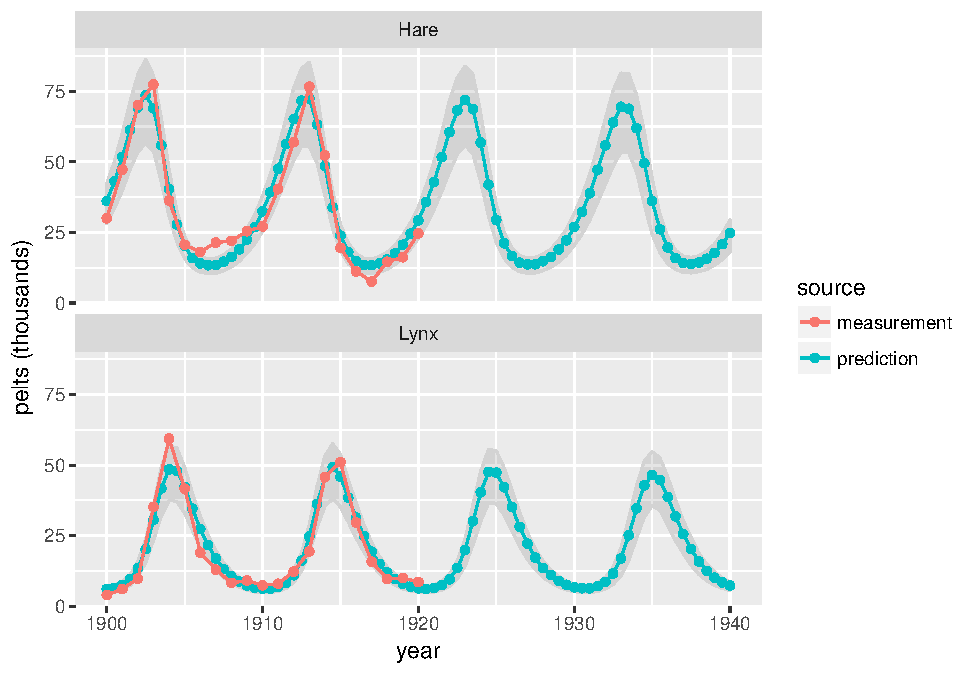
\includegraphics[width=0.525\textwidth]{img/lotka-volterra-predict.pdf}
\end{center}
\vspace*{-6pt}
\begin{subsubitemize}
\item did not include \texttt{generated quantities} block---just more of same
\item training data (1900-1920); \ future predictions (1921+)
\end{subsubitemize}


\sld{Platforms and Interfaces}
%
\vspace*{-2pt}
\begin{itemize}
\item \myemph{Platforms}:  Linux, Mac OS X, Windows
\item \myemph{C++ API}: {\small portable, standards compliant (C++11)}
\item \myemph{Interfaces}
\begin{subitemize}\footnotesize
  \item \myemph{CmdStan}: Command-line or shell interface (direct executable)
  \item \myemph{RStan}: R interface (Rcpp in memory)
  \item \myemph{PyStan}: Python interface (Cython in memory)
  \item \myemph{MatlabStan}: MATLAB interface (external process)
  \item \myemph{Stan.jl}: Julia interface (external process)
  \item \myemph{StataStan}: Stata interface (external process)
  \item \myemph{MathematicaStan}: Stata interface (external process)
\end{subitemize}
\end{itemize}


\sld{Higher-Level Interfaces}
%
\begin{subitemize}
\item \myemph{R Interfaces}
\begin{subsubitemize}
 \item \myemph{RStanArm}: regression modeling with R expressions
 \item \myemph{ShinyStan}: web-based posterior visualization, exploration
 \item \myemph{Loo}:  approximate leave-one-out cross-validation
\end{subsubitemize}
\item \myemph{Jupyter Containers}
\begin{subsubitemize}
\item \myemph{Docker} versions for R, Python, Julia
\item \myemph{SageMath}: free online server (R)
\end{subsubitemize}
\item From others
\begin{subsubitemize}
\item \myemph{Prophet} (Facebook): time-series analysis (R and Python)
\item \myemph{brms} (B\"urkner): regression modeling with R expressions
\item \myemph{rethinking} (McElreath): simplified Stan embedded in R
\end{subsubitemize}
\end{subitemize}


\sld{\Large Who's Using Stan?}
%
\begin{subitemize}
\item 100,000+ ``\myemph{users}'';  7500+ \myemph{users group} registrations;  millions \myemph{downloads}; 10,000+ Google scholar citations
\item \myemph{Biological sciences}: {\footnotesize
clinical drug trials, entomology, pharmacology, toxicology, botany,
neurology, genomics, agriculture, botany, fisheries, genomics, cellular
biology, epidemiology, population ecology
}
\item \myemph{Physical sciences}: {\footnotesize
astrophysics, particle physics, molecular biology, oceanography, climatology, biogeochemistry, materials science
}
\item \myemph{Social sciences}: {\footnotesize
 econometrics (macro and micro), population dynamics, cognitive
 science, psycholinguistics, social networks, political science,
 survey sampling
}
\item \myemph{Other}: {\footnotesize materials engineering, finance,
    actuarial science, sports, public health, recommender systems,
    education, fleet maintenance}
\end{subitemize}


\sld{Documentation}
%
\begin{itemize}
\item {\slshape Stan User's Guide}, {\slshape Stan Reference Manual}, and {\slshape Stan Functions Reference}.
\begin{subitemize}
\item example models, modeling and programming advice
\item introduction to Bayesian and frequentist statistics
\item complete language specification and execution guide
\item descriptions of algorithms (NUTS, R-hat, n\_eff)
\item guide to built-in distributions and functions
\end{subitemize}
\item {\slshape Installation, Getting Started, Documentation} by interface
\begin{subitemize}
\item Algorithms: CmdStanR, CmdStanPy, RStan, PyStan, CmdStan, MatlabStan, Stan.jl, StataStan, MathematicaStan
\item Model: BridgeStan interfaces in R, Python, Julia, Rust, C, and C++
\end{subitemize}
\item Dozens of written and video tutorials by users and developers
\end{itemize}


\sld{Model Sets Translated to Stan}
%
\begin{itemize}
\item BUGS examples (most of all 3 volumes)
\item Gelman and Hill (2009) {\slshape Data Analysis Using Regression and
    Multilevel/Hierarchical Models}.
\item Wagenmakers and Lee (2014) {\slshape Bayesian Cognitive
    Modeling}.
\item K\'ery and Schaub (2014) {\slshape Bayesian Population Analysis
    Using WinBUGS}.
\item Kruschke (2014) {\slshape Doing Bayesian Data Analysis}.
\end{itemize}

\sld{Books about and using Stan}
%
{\footnotesize
\begin{itemize}
\item Gelman and Vehtari (2025) {\slshape Active
    Statistics}. Cambridge.
\item Marc K\'ery and Kenneth F. Kellner (2024)
{\slshape Applied Statistical Modelling for Ecologists: A Practical
  Guide to Bayesian and Likelihood Inference Using R, JAGS, NIMBLE,
  Stan and TMB.} Elsevier.  
\item Suzuki, J. (2023) {\slshape WAIC and WBIC with R Stan: 100
    Exercises for Building Logic}. Springer.
\item Song S. Qian, Mark R. DuFour and Ibrahim Alameddine. (2022)
  {\slshape Bayesian Applications in Environmental and Ecological
    Studies with R and Stan}. CRC.  
\item Matsuura, K. (2022) {\slshape Bayesian Statistical Modeling with Stan, R, and Python}. Springer.
\item Jin Xu. (2022) {\slshape Modern Applied Regressions: Bayesian and Frequentist Analysis of Categorical and Limited Response Variables with R and Stan}. CRC.
  \item Rudolf Debelak, Carolin Strobl, and Matthew D. Zeigenfuse. (2022) {\slshape An Introduction to the Rasch Model with Examples in R.} CRC.
  \item Marco Scutari and Jean-Baptiste Denis. (2021) {\slshape Bayesian Networks With Examples in R}. Second Edition. CRC.
\item Johnson, A.A., M. Q. Ott, M. Dogucu. (2021) {\slshape Bayes Rules! An Introduction to Applied Bayesian Modeling.} CRC Press.
\item Nick Heard. (2021) {\slshape An Introduction to Bayesian Inference, Methods, and Computation}. Springer.
\item Richard McElreath (2020) {\slshape Statistical Rethinking: A Bayesian course 
    with R and Stan}. CRC. Second Edition.  
\item Andrew Gelman, Aki Vehtari, and Jennifer Hill (2020) {\slshape Regression and Other Stories}. Cambridge.
  \item Harray Yang and Steven J. Novick. (2019) {\slshape Bayesian Analysis with R for Drug Development: Concepts, Algorithms, and Case Studies.} CRC.
\item Peter D. Congdon. (2019) {\slshape Bayesian Hierarchical Models with Applications Using R}. Second Edition. CRC.
\item Holmes, E. E., M. D. Scheuerell, and E. J. Ward. (2019). {\slshape 
    Applied Time Series Analysis for Fisheries and Environmental Sciences}. NOAA Fisheries, Northwest Fisheries Science Center.
\item Guangyuan Guo. (2019) {\slshape Bayesian Claims Reserving Methods in Non-life Insurance with Stan: An Introduction}. Springer.
\item Jaroslaw Harezlak,
David Ruppert, and Matt P. Wand. (2018) {\slshape Semiparametric Regression with R}. Springer.
\item Lambert, Ben.  (2018) {\slshape A Student's Guide to Bayesian 
    Statistics}. 
\item Hilbe, de Souza, and Ishida (2017) {\slshape Bayesian Models for Astrophysical Data Using R, JAGS, Python, and Stan}. Cambridge. 
\item Matsuura (2016) {\slshape Bayesian Statistical Modeling Using Stan and R}. Kyoritsu. (Japanese) 
\item McElreath (2016) {\slshape Statistical Rethinking: A Bayesian course 
    with R and Stan}. CRC. 
\item Faraway (2016) {\slshape Extending the Linear Model with R: Generalized Linear, Mixed Effects and Nonparametric Regression Models}, 2nd Edition. CRC.
\item Korner-Nievergelt et al. (2015) {\slshape Bayesian Data Analysis in
    Ecology Using Linear Models with R, BUGS, and Stan}. Academic Press.
\item Kruschke (2014) {\slshape Doing Bayesian Data Analysis, Second
    Edition: A Tutorial with R, JAGS, and Stan}. Academic Press.
\item Gelman et al. (2013) {\slshape Bayesian Data Analysis}, 3rd Edition. CRC.
\end{itemize}
}


\sld{Stan is a Programming Language}
%
\begin{itemize}
\item \myemph{Not} a graphical specification language like BUGS, JAGS, PyMC, NumPyro, etc.
\item Stan is a \myemph{Turing-complete} imperative programming language for specifying differentiable log densities
\begin{subitemize}
\item reassignable local variables and scoping
\item full conditionals and loops
\item functions (including recursion)
\end{subitemize}
\item Stan layers automatic ``black-box'' inference on top
\item Programs computing same thing may have different efficiency
\end{itemize}


\sld{Basic Program Blocks}
%
\begin{itemize}
\item \myemph{\tt\bfseries data} \ (once)
  \vspace*{-4pt}
  \begin{itemize}\small
  \item {\slshape content}: declare data types, sizes, and constraints
  \item {\slshape execute}: read from data source, validate constraints
  \end{itemize}
  %
\item \myemph{\tt\bfseries parameters} \ (every log prob eval)
  \vspace*{-4pt}
  \begin{itemize}\small
  \item {\slshape content}: declare parameter types, sizes, and constraints
  \item {\slshape execute}: transform to constrained, Jacobian
  \end{itemize}
  %
\item \myemph{\tt\bfseries model} \ (every log prob eval)
  \vspace*{-4pt}
  \begin{itemize}\small
  \item {\slshape content}: statements defining posterior density
  \item {\slshape execute}: execute statements
  \end{itemize}
\end{itemize}


\sld{Derived Variable Blocks}
%
\begin{itemize}
\item \myemph{\tt\bfseries transformed data} (once after data)
  \vspace*{-4pt}
  \begin{itemize}\small
  \item {\slshape content}: declare and define transformed data variables
  \item {\slshape execute}: execute definition statements, validate constraints
  \end{itemize}
  %
\item \myemph{\tt\bfseries transformed parameters} (every log prob eval)
  \vspace*{-4pt}
  \begin{itemize}\small
  \item {\slshape content}: declare and define transformed parameter vars
  \item {\slshape execute}: execute definition statements, validate constraints
  \end{itemize}
  %
\item \myemph{\tt\bfseries generated quantities} (once per draw,
  \code{double} type)
  \vspace*{-4pt}
  \begin{itemize}\small
  \item {\slshape content}: declare and define generated quantity
    variables; \\
    includes pseudo-random number generators
    \\
    {\footnotesize (for posterior predictions, event probabilities,
      decision making)}
  \item {\slshape execute}: execute definition statements, validate constraints
  \end{itemize}
  %
\end{itemize}


\sld{Model: Read and Transform Data}
%
\begin{itemize}
\item Only done once for optimization or sampling (per chain)
\item Read data
\begin{subitemize}
\item read data variables from memory or file stream
\item validate data
\end{subitemize}
\item Generate transformed data
\begin{subitemize}
\item execute transformed data statements
\item validate variable constraints when done
\end{subitemize}
\end{itemize}


\sld{Model: Log Density}
%
\begin{itemize}
\item \emph{Given} parameter values on unconstrained scale
\item Builds \myemph{expression graph} for log density (start at 0)
\item \myemph{Inverse transform} unconstrained parameters to constrained scale
\begin{subitemize}
\item constraints involve non-linear transforms
\item e.g.,  positive constrained $x$ to unconstrained $y = \log x$
\end{subitemize}
\item account for curvature in change of variables
\begin{subitemize}
\item e.g., unconstrained $y$ to positive $x = \log^{-1}(y) =
  \exp(y)$
\item e.g., add \myemph{log Jacobian determinant}, $\log |\frac{d}{dy} \exp(y)| = y$
\end{subitemize}
\item \myemph{Execute model block} statements to increment log density
\end{itemize}

\sld{Model: Log Density Gradient}
%
\begin{itemize}
\item Log density evaluation builds up expression graph
\begin{subitemize}
\item templated overloads of functions and operators
\item efficient arena-based memory management
\end{subitemize}
\item Compute gradient in backward pass on expression graph
\begin{subitemize}
\item propagate partial derivatives via chain rule
\item work backwards from final log density to parameters
\item dynamic programming for shared subexpressions
\item very memory intensive (about 40 bytes/operation)
\end{subitemize}
\item Linear multiple of time to evaluate log density (3--5 times)
\end{itemize}


\sld{Model: Generated Quantities}
%
\begin{itemize}
\item \myemph{Given} parameter values
\item Once per iteration (not once per leapfrog step)
\item May involve (pseudo) random-number generation
\begin{subitemize}
\item Executed generated quantity statements
\item Validate values satisfy constraints
\end{subitemize}
\item Typically used for
\begin{subitemize}
\item Event probability estimation
\item Predictive posterior estimation
\end{subitemize}
\item Efficient because evaluated with \code{double} types (no autodiff)
\end{itemize}


\sld{Variable Transforms}
%
\begin{itemize}
\item Code HMC and optimization with $\mathbb{R}^n$ \myemph{support}
\item Transform constrained parameters to unconstrained
  \vspace*{-2pt}
  {\small
    \begin{itemize}
    \item lower (upper) bound: offset (negated) log transform
    \item lower and upper bound: scaled, offset logit transform
    \item simplex: centered, stick-breaking logit transform (moving to ILR)
    \item ordered: free first element, log transform offsets
    \item unit length: sample from overparameterized standard normal and project
    \item covariance matrix: Cholesky factor positive diagonal
    \item correlation matrix: rows unit length via quadratic stick-breaking
    \item sum-to-zero: uses first part isometric log ratio (ILR) transform
    \end{itemize}
  }
\end{itemize}


\sld{Variable Transforms (cont.)}
%
\begin{itemize}
\item Inverse transform from unconstrained $\mathbb{R}^n$
\item Evaluate log probability in model block on natural scale
\item Optionally adjust log probability for change of variables
\begin{subitemize}
\item adjustment for MCMC and variational, not MLE
\item add log determinant of inverse transform Jacobian
\item automatically differentiable
\end{subitemize}
\end{itemize}


\sld{Variable and Expression Types}
%
\\[3pt]
\hspace*{17pt}Variables and expressions are \myemph{strongly, statically typed}.
\begin{itemize}
\item \myemph{Primitive}: {\tt\small int}, \ {\tt\small real}
\item \myemph{Matrix}: {\tt\small matrix[M,N]}, \ {\tt\small vector[M]}, \ {\tt\small row\_vector[N]}
\item \myemph{Bounded}: primitive or matrix, with
  \\ {\tt\small <lower=L>}, \ {\tt\small <upper=U>}, \ {\tt\small <lower=L,upper=U>}
\item \myemph{Constrained Vectors}: {\tt\small simplex[K]}, \ {\tt\small
    ordered[N]},
  \\ {\tt\small positive\_ordered[N]}, \ {\tt\small unit\_length[N]}
\item \myemph{Constrained Matrices}: {\tt\small cov\_matrix[K]}, \ {\tt\small
    corr\_matrix[K]}, \\ {\tt\small cholesky\_factor\_cov[M,N]}, \
  {\tt\small cholesky\_factor\_corr[K]}
\item \myemph{Arrays:}  of any type (and dimensionality)
\end{itemize}


\sld{Integers vs.\ Reals}
%
\begin{itemize}
\item Different types (conflated in BUGS, JAGS, and R)
\item Distributions and assignments care
\item Integers may be assigned to reals but not vice-versa
\item Reals have not-a-number, and positive and negative infinity
\item Integers single-precision up to +/- 2 billion
\item Integer division rounds (Stan provides warning)
\item Real arithmetic is inexact and reals should not be (usually) compared with \code{==}
\end{itemize}


\sld{Arrays vs. Vectors \& Matrices}
%
\begin{itemize}
\item Stan separates arrays, matrices, vectors, row vectors 
  \begin{subitemize}
    \item should have followed NumPy's overloading, but typing gives easy reductions (e.g., matrix times vector is vector)
  \end{subitemize}
\item Arrays allow most efficient access (no copying)
\item Arrays stored first-index major (i.e., 2D are row major)
\item Vectors and matrices required for matrix and linear algebra functions
\item Matrices stored column-major (memory locality matters)
\item Are not assignable to each other, but there are conversion functions
\end{itemize}


\sld{Logical Operators}
%
\vfill
\noindent\spc
{\footnotesize
  \begin{tabular}{c|ccl|l}
    {\it Op.} & {\it Prec.} & {\it Assoc.} & {\it
      Placement} & {\it Description}
    \\ \hline \hline
    \code{||} & 9 & left & binary infix & logical or
    \\ \hline
    \Verb|&&| & 8 & left & binary infix & logical and
    \\ \hline
    \Verb|==| & 7 & left & binary infix & equality
    \\
    \Verb|!=| & 7 & left & binary infix & inequality
    \\ \hline
    \Verb|<| & 6 & left & binary infix & less than
    \\
    \Verb|<=| & 6 & left & binary infix & less than or equal
    \\
    \Verb|>| & 6 & left & binary infix & greater than
    \\
    \Verb|>=| & 6 & left & binary infix & greater than or equal
  \end{tabular}
}
\vfill
\vfill


\sld{Arithmetic and Matrix Operators}
%
\vfill
\noindent\spc
{\footnotesize
  \begin{tabular}{c|ccl|l}
    {\it Op.} & {\it Prec.} & {\it Assoc.} & {\it
      Placement} & {\it Description}
    \\ \hline \hline

    \code{+} & 5 & left & binary infix & addition
    \\
    \code{-} & 5 & left & binary infix & subtraction
    \\ \hline
    \code{*} & 4 & left & binary infix & multiplication
    \\
    \code{/} & 4 & left & binary infix & (right) division
    \\ \hline
    \Verb|\| & 3 & left & binary infix & left division
    \\ \hline
    \code{.*} & 2 & left & binary infix & elementwise multiplication
    \\
    \code{./} & 2 & left & binary infix & elementwise division
    \\ \hline
    \code{!} & 1 & n/a & unary prefix & logical negation
    \\
    \code{-} & 1 & n/a & unary prefix & negation
    \\
    \code{+} & 1 & n/a & unary prefix & promotion (no-op in Stan)
    \\ \hline
    \Verb|^| & 2 & right & binary infix & exponentiation
    \\ \hline
    \code{'} & 0 & n/a & unary postfix & transposition
    \\ \hline \hline
    \code{()} & 0 & n/a & prefix, wrap & function application
    \\
    \code{[]} & 0 & left & prefix, wrap & array, matrix indexing
  \end{tabular}
}


\sld{Assignment Operators}
%
\null \\
\spc{\footnotesize
  \begin{tabular}{c|ccl|l}
    {\it Op.} & {\it Description} \\ \hline \hline
    \code{=} & assignment \\
    \code{+=} & compound add and assign \\
    \code{-=} & compound subtract and assign \\
    \code{*=} & compound multiply and assign \\
    \code{/=} & compound divide and assign \\
    \code{.*=} & compound elementwise multiply and assign \\
    \code{./=} & compound elementwise divide and assign \\

  \end{tabular}
}
%
\begin{itemize}
\item these work with all relevant matrix types
\begin{subitemize}
\item e.g., \Verb|matrix *= matrix;|
\end{subitemize}
\end{itemize}


\sld{Built-in Math Functions}
%
\begin{itemize}
\item All built-in \myemph{C++ functions and operators}
  \\
  {\footnotesize C math, TR1, C++11, including all trig, pow, and
    special log1m, erf, erfc, fma, atan2, etc.}
\item Extensive library of \myemph{statistical functions}
  \\
  {\footnotesize e.g., softmax,
    log gamma and digamma functions, beta functions, Bessel functions of
    first and second kind, etc.}
  %
\item Efficient, arithmetically stable \myemph{compound functions}
  \\
  {\footnotesize e.g., multiply log, log sum of
    exponentials, log inverse logit}
\end{itemize}


\sld{Built-in Matrix Functions}
%
\begin{itemize}\small
\item \myemph{Basic arithmetic}: all arithmetic operators
\item \myemph{Elementwise arithmetic}: vectorized operations
\item \myemph{Solvers}: matrix division, (log) determinant,
  inverse
\item \myemph{Decompositions}: QR, Eigenvalues and Eigenvectors,
  \\
  Cholesky factorization, singular value decomposition
\item \myemph{Compound Operations}: quadratic forms, variance scaling, etc.
\item \myemph{Ordering, Slicing, Broadcasting}: sort, rank, block, rep
\item \myemph{Reductions}: sum, product, norms
\item \myemph{Specializations}: triangular, positive-definite,
\end{itemize}


\sld{Atomic Statements}
%
\begin{itemize}
\item \myemph{Distribution}: \ {\footnotesize \Verb|y ~ normal(mu,sigma)|}
  \ \ \ {\footnotesize (syntactic sugar: just \myemph{increments log probability})}
\item \myemph{Increment log density}: \ {\footnotesize target += lp;}
\item \myemph{Assignment}: \  {\footnotesize \code{y\_hat = x * beta};}
\end{itemize}


\sld{Block of Statements}
%
\begin{itemize}
\item \myemph{Block}: \ {\footnotesize \Verb|{ ...; ...; ...; }|}
  \hfill {\footnotesize
    (allows initial local variables)}
\end{itemize}

\sld{Control Statements}
%
\begin{itemize}
\item \myemph{For loop}: \ {\footnotesize \code{for (n in 1:N) ...}}
\item \myemph{While loop}: \ {\footnotesize \code{while (cond) ...}}
\item \myemph{Conditional}: \ {\footnotesize
    \code{if (cond) ...; else if (cond) ...;  else ...;}}
\item \myemph{Break}: \ {\footnotesize \code{break}}
\item \myemph{Continue}: \ {\footnotesize \code{continue}}
\end{itemize}

\sld{Side-Effect Statements}
%
\begin{itemize}
\item \myemph{Print}: \ {\footnotesize \code{print("theta=", theta);}}
\item \myemph{Reject}:
\ {\footnotesize
    \code{reject("arg to foo must be positive, found y=", y);}}
\end{itemize}


\sld{``Sampling'' Increments Log Prob}
%
\begin{itemize}
\item A Stan program defines a log posterior
\begin{subitemize}
\item typically through log joint and Bayes's rule
\end{subitemize}
\item Sampling statements are just ``syntactic sugar''
\item A shorthand for incrementing the log posterior
\item The following define the same$^*$ posterior
\begin{itemize}
\item \Verb|y ~ poisson(lambda);|
\item \Verb|target += poisson_lpmf(y, lambda);|
\end{itemize}
\item ${}^{*}$ up to a constant
\item Sampling statement drops constant terms
\end{itemize}



\sld{Local Variable Scope Blocks}
%
\begin{itemize}
\item
\begin{Verbatim}
  y ~ bernoulli(theta);
\end{Verbatim}
is more efficient with sufficient statistics
{\small
\begin{Verbatim}
  {
    real sum_y;  // local variable
    sum_y = 0;
    for (n in 1:N)
      sum_y = sum_y + y[n];   // reassignment
    sum_y ~ binomial(N, theta);
  }
\end{Verbatim}
}
\item Simpler, but roughly same efficiency:
\begin{Verbatim}
    sum(y) ~ binomial(N, theta);
\end{Verbatim}
\end{itemize}


\sld{User-Defined Functions}
%
\begin{itemize}
\item \myemph{\tt\bfseries functions} \ (compiled with model)
  \vspace*{-4pt}
  \begin{itemize}\small
  \item {\slshape content}: declare and define general (recursive) functions
    \\
    {\small (use them elsewhere in program)}
  \item {\slshape execute}: compile with model
  \end{itemize}
  \vspace*{6pt}
\item Example
  \\[6pt]
  \begin{minipage}[t]{0.8\textwidth}
    \footnotesize
    \begin{Verbatim}
      functions {

        real relative_difference(real u, real v) {
          return 2 * fabs(u - v) / (fabs(u) + fabs(v));
        }

      }
    \end{Verbatim}
  \end{minipage}
\end{itemize}

\sld{Special User-Defined Functions}
%
\begin{itemize}
\item When declared with appropriate naming, user-defined functions
  may
\begin{subitemize}
\item be used in sampling statements: \code{real} return and suffix \Verb|_lpdf| or \Verb|_lpmf|
\item use RNGs: suffix \Verb|_rng|
\item use target accumulator:  suffix \Verb|_lp|
\end{subitemize}
\end{itemize}


\sld{User-Defined PDFs and CDFs}
%
\begin{itemize}
\item May be used with sampling and PDF/PMF notation
\begin{subitemize}
\item \myemph{density}: suffix \code{\_lpdf} if variate (first arg) is real
\item \myemph{mass}: Suffix \code{\_lpmf} if variate (first arg) is integer
\end{subitemize}
\end{itemize}
%
{\small
\begin{stancode}
functions {
  real centered_normal_lpdf(real y, real sigma) {
    return -0.5 * (y / sigma)^2;
  }

model {
  y ~ centered_normal(2.5);                 // sampling

  target += centered_normal_lpdf(y | 2.5);  // pdf notation
\end{stancode}
}


\sld{Target Incrementing Functions}
%
\begin{itemize}
\item Only usable in model block
\begin{subitemize}
\item must end in \code{\_lp}
\end{subitemize}
\end{itemize}
%
\begin{stancode}
functions {
  vector non_center_lp(vector beta_std, real mu, real sigma) {
    beta_std ~ normal(0, 1);
    return mu + sigma * beta_raw;
  }
parameters {
  vector[K] beta_std;
model {
  vector[K] beta = non_center_lp(beta_std);
  y ~ normal(x * beta, sigma);
\end{stancode}


\sld{RNG Functions}
%
\begin{itemize}
\item Only usable in generated quantities block
\begin{subitemize}
\item must end in \code{\_rng}
\end{subitemize}
\end{itemize}
%
\begin{stancode}
functions {
  real centered_normal_rng(real sigma) {
    return normal_rng(0, sigma);
  }

generated quantities {
  real alpha = centered_normal_rng(2.7);
\end{stancode}



\sld{Differential Equation Solver}
%
\begin{itemize}
\item System expressed as function
\begin{subitemize}
\item given state ($y$) time ($t$), parameters ($\theta$), and data ($x$)
\item return derivatives ($\partial y / \partial t$) of state w.r.t. time
\end{subitemize}
\item Simple harmonic oscillator diff eq
\begin{stancode}
  real[] sho(data real t,        // time
             real[] y,           // system state
             real[] theta,       // params
             data real[] x_r,    // real data
             data int[] x_i) {   // int data
    return { y[2],
             -y[1] - theta[1] * y[2] };
 }
\end{stancode}
\end{itemize}


\sld{Differential Equation Solver (cont.)}
%
\begin{itemize}
\item Solution via functional, given initial state (\code{y0}),
initial time (\code{t0}), desired solution times (\code{ts})
{\footnotesize
\begin{Verbatim}
  mu_y = integrate_ode(sho, y0, t0, ts, theta, x_r, x_i);
\end{Verbatim}
}
\item Use noisy measurements of $y$ to estimate $\theta$
\begin{Verbatim}
y ~ normal(mu_y, sigma);
\end{Verbatim}
\begin{subitemize}
\item Pharmacokinetics/pharmacodynamics (PK/PD),
\item soil carbon respiration with biomass input and breakdown
\end{subitemize}
\end{itemize}


\sld{Built-in Diff Eq Solvers}
%
\begin{itemize}
\item \myemph{Non-stiff solver}: Runge-Kutta 4th/5th order (RK45)
\item \myemph{Stiff solver}:  backward-differentiation formula (BDF)
\begin{subitemize}
\item slower
\item more robust for derivatives of different scales or high
  curvature
\end{subitemize}
\item specified by suffix \Verb|_bdf| or \Verb|_rk45|
\end{itemize}


\sld{Diff Eq Derivatives}
%
\begin{itemize}
\item User defines system $\frac{\partial}{\partial t} y$
\item Need derivatives of solution $y$ w.r.t.\ parameters $\theta$
\item Couple derivatives of system  w.r.t. parameters
\[
\left(
\frac{\partial}{\partial t} \, y, \ \
\frac{\partial}{\partial t} \, \frac{\partial}{\partial \theta} \, y
\right)
\]
\item Calculate coupled system via nested autodiff of second term
\[
\frac{\partial}{\partial t} \, \frac{\partial}{\partial \theta} \, y
\ = \
\frac{\partial}{\partial \theta} \, \frac{\partial}{\partial t} \, y.
\]
\item Originally coupled this way, now also use \myemph{adjoint methods}
\end{itemize}

\sld{Other built-in Solvers}
\begin{itemize}
\item Differential algebraic equation solver (e.g., for economic equilibrium models)
\item One-dimensional integrator (e.g., for defining cdfs)
\item Root finder (e.g., for defining inverse cdfs) 
\item Hidden Markov models (use forward/backward algorithm)
  \vfill
\item Gradients all through the implicit function theorem.
\end{itemize}

\sld{Distribution Library}
%
\begin{itemize}
\item Each distribution has
  \vspace*{-4pt}
  \begin{itemize}\small
  \item log density or mass function
  \item cumulative distribution functions, plus complementary versions,
    plus log scale
  \item Pseudo-random number generators
  \end{itemize}
\item Alternative parameterizations
  \\
  {\footnotesize (e.g., Cholesky-based multi-normal,
    log-scale Poisson, logit-scale Bernoulli)}
\item New multivariate correlation matrix density: LKJ
  \\
  {\footnotesize degrees of freedom controls
    shrinkage to (expansion from) unit matrix}
\end{itemize}


\sld{Print and Reject}
%
\begin{itemize}
\item Print statements are for \myemph{debugging}
\begin{subitemize}
\item printed every log prob evaluation
\item print values in the middle of programs
\item check when log density becomes undefined
\item can embed in conditionals
\end{subitemize}
\item Reject statements are for \myemph{error checking}
\begin{subitemize}
\item typically function argument checks
\item cause a rejection of current state (0 density)
\end{subitemize}
\end{itemize}


\sld{Probability Function Vectorization}
%
\begin{itemize}
\item Stan's probability functions are vectorized for speed
\begin{subitemize}
\item removes repeated computations (e.g., $-\log \sigma$ in normal)
\item reduces size of expression graph for differentiation
\end{subitemize}
\item Consider: \ \Verb|y ~ normal(mu, sigma);|
\item Each of \code{y}, \code{mu}, and \code{sigma} may be any of
\begin{subitemize}
\item scalars (integer or real)
\item vectors (row or column)
\item 1D arrays
\end{subitemize}
\item All dimensions must be scalars or having matching sizes
\item Scalars are broadcast (repeated)
\end{itemize}


\sld{Parsing and Compilation}
%
\begin{itemize}
\item Stan code \myemph{parsed} to abstract syntax tree (AST)
  \\ {\footnotesize (Boost Spirit Qi, recursive descent, lazy semantic
    actions)}
\item C++ model class \myemph{code generation} from AST
  \\ {\footnotesize (Boost Variant)}
\item C++ code \myemph{compilation}
\item \myemph{Dynamic linking} for RStan, PyStan
\end{itemize}



\sld{Euclidean Hamiltonian Monte Carlo}
%
\begin{itemize}
\item \myemph{Phase space}: $q$ position (parameters); \ $p$ momentum
\item \myemph{Posterior density}: $\pi(q)$
\item \myemph{Mass matrix}: $M$
\item \myemph{Potential energy}: $V(q) = -\log \pi(q)$
\item \myemph{Kinetic energy}: $T(p) = \frac{1}{2} p^{\top} M^{-1} p$
\item \myemph{Hamiltonian}:  $H(p,q) = V(q) + T(p)$
\item \myemph{Diff eqs}:
  \[
  \frac{dq}{dt} \ = \  + \frac{\partial H}{\partial p}
  \hspace*{48pt}
  \frac{dp}{dt} \ = \ - \frac{\partial H}{\partial q}
  \]
\end{itemize}


\sld{Leapfrog Integrator Steps}
%
\begin{itemize}
\item Solves Hamilton's equations by \myemph{simulating dynamics}
  \\
  {\footnotesize (symplectic [volume preserving]; $\epsilon^3$ error per step, $\epsilon^2$ total error)}
\item Given: \myemph{step size} $\epsilon$, \myemph{mass matrix} $M$, \myemph{parameters} $q$
\item \myemph{Initialize kinetic} energy, $p \sim {\sf
    Normal}(0,\mbox{\bf I})$
\item \myemph{Repeat} for $L$ leapfrog steps:
  \begin{eqnarray*}
    p & \leftarrow &
    p - \frac{\epsilon}{2} \, \frac{\partial V(q)}{\partial q}
    \ \ \ \ \ \ \mbox{[half step in momentum]}
    \\[6pt]
    q & \leftarrow &
    q + \epsilon \, M^{-1} \, p
    \ \ \ \ \ \ \ \  \mbox{[full step in position]}
    \\[6pt]
    p & \leftarrow &
    p - \frac{\epsilon}{2} \, \frac{\partial V(q)}{\partial q}
    \ \ \ \ \ \ \mbox{[half step in momentum]}
  \end{eqnarray*}
\end{itemize}


\sld{Adaptation During Warmup}
%
\begin{itemize}
\item (I) initial fast interval to find typical set with unit mass matrix
\\
(step size,   default 75 iterations)
\begin{subitemize}
\item Adrian Seyboldt's Nutpie uses abs.\ val.\ of gradient to initialize
  \item absolute value is geometric mean of unit and outer product of gradients 
  \end{subitemize}
\item (II) expanding memoryless windows to estimate metric; doubles each time and re-estimates mass matrix from draws
\\
(step size \& metric, initial window 25 iterations; total 875)
\begin{subitemize}
  \item Seyboldt showed improvement with geometric mean of empirical estimate from draws and inverse of empirical estimate of precision from covariance of scores.
\end{subitemize}
\item (III) final fast interval to tune step size
  \\
  (step size, default 50 iterations)
\end{itemize}


\sld{Laplace Approximation}
%
\begin{itemize}
\item Multivariate normal approximation to posterior
\item Compute posterior mode via optimization
\[
\theta^{*} = \argmax_{\theta} \  p(\theta | y)
\]
\item Laplace approximation to the posterior is
\[
p(\theta | y)
\approx
\distro{MultiNormal}(\theta^{*} | -H^{-1}(\theta^*))
\]
\item $H$ is the Hessian of the log posterior
\[
H_{i,j}
= \frac{\partial^2}{\partial \theta_i \ \partial \theta_j}
  \log p(\theta | y)
\]
\end{itemize}


\sld{Stan's Laplace Approximation}
%
\begin{itemize}
\item Operates on unconstrained parameters
\item L-BFGS to compute posterior mode $\theta^*$
\item Automatic differentiation to compute $H$
\begin{subitemize}
\item current R: finite differences of gradients
\item soon:  second-order automatic differentiation
\end{subitemize}
\item Draw a sample from approximate posterior
\begin{subitemize}
\item transfrom back to constrained scale
\item allows Monte Carlo computation of expectations
\end{subitemize}
\end{itemize}


\sld{``Black Box'' Variational Inference}
%
\begin{itemize}
%
\item \myemph{Black box} so can fit any Stan model
%
\item Multivariate \myemph{normal approx to unconstrained} posterior
\begin{subitemize}
\item covariance: diagonal mean-field or full rank
\item not Laplace approx --- around posterior mean, not mode
\item transformed back to constrained space (built-in Jacobians)
\end{subitemize}
%
\item Stochastic \myemph{gradient-descent} optimization
\begin{subitemize}
\item ELBO gradient estimated via Monte Carlo + autodiff
\end{subitemize}
%
\item Returns \myemph{approximate posterior} mean / covariance
\item Returns \myemph{sample} transformed to constrained space
\end{itemize}


\sld{VB in a Nutshell}
%
\begin{itemize}
\item $y$ is observed data, $\theta$ parameters
\item Goal is to approximate posterior $p(\theta | y)$
\item with a convenient approximating density $g(\theta | \phi)$
\begin{subitemize}
\item $\phi$ is a vector of parameters of approximating density
\end{subitemize}
\item Given data $y$, VB computes $\phi^*$
minimizing KL-divergence
{\small
\begin{eqnarray*}
\phi^*
& = &
\displaystyle
\argmin_{\phi} \ \mbox{KL}[g(\theta|\phi) \ || \ p(\theta|y)]
\\[4pt]
& = &
\displaystyle
\argmin_{\phi}
\int_{\Theta}
  \log\left(
    \frac{p(\theta \, | \, y)}{g(\theta \, | \, \phi)}
  \right)
  \ g(\theta | \phi) \ \mathrm{d}\theta
\\[4pt]
& = &
\argmin_{\phi} \
\mathbb{E}_{g(\theta|\phi)}\left[\,
  \log p(\theta \, | \, y) - \log g(\theta \, | \, \phi)
\right]
\end{eqnarray*}
}
\end{itemize}


\sld{VB vs.\ Laplace}
%
\vspace*{-6pt}
\begin{center}
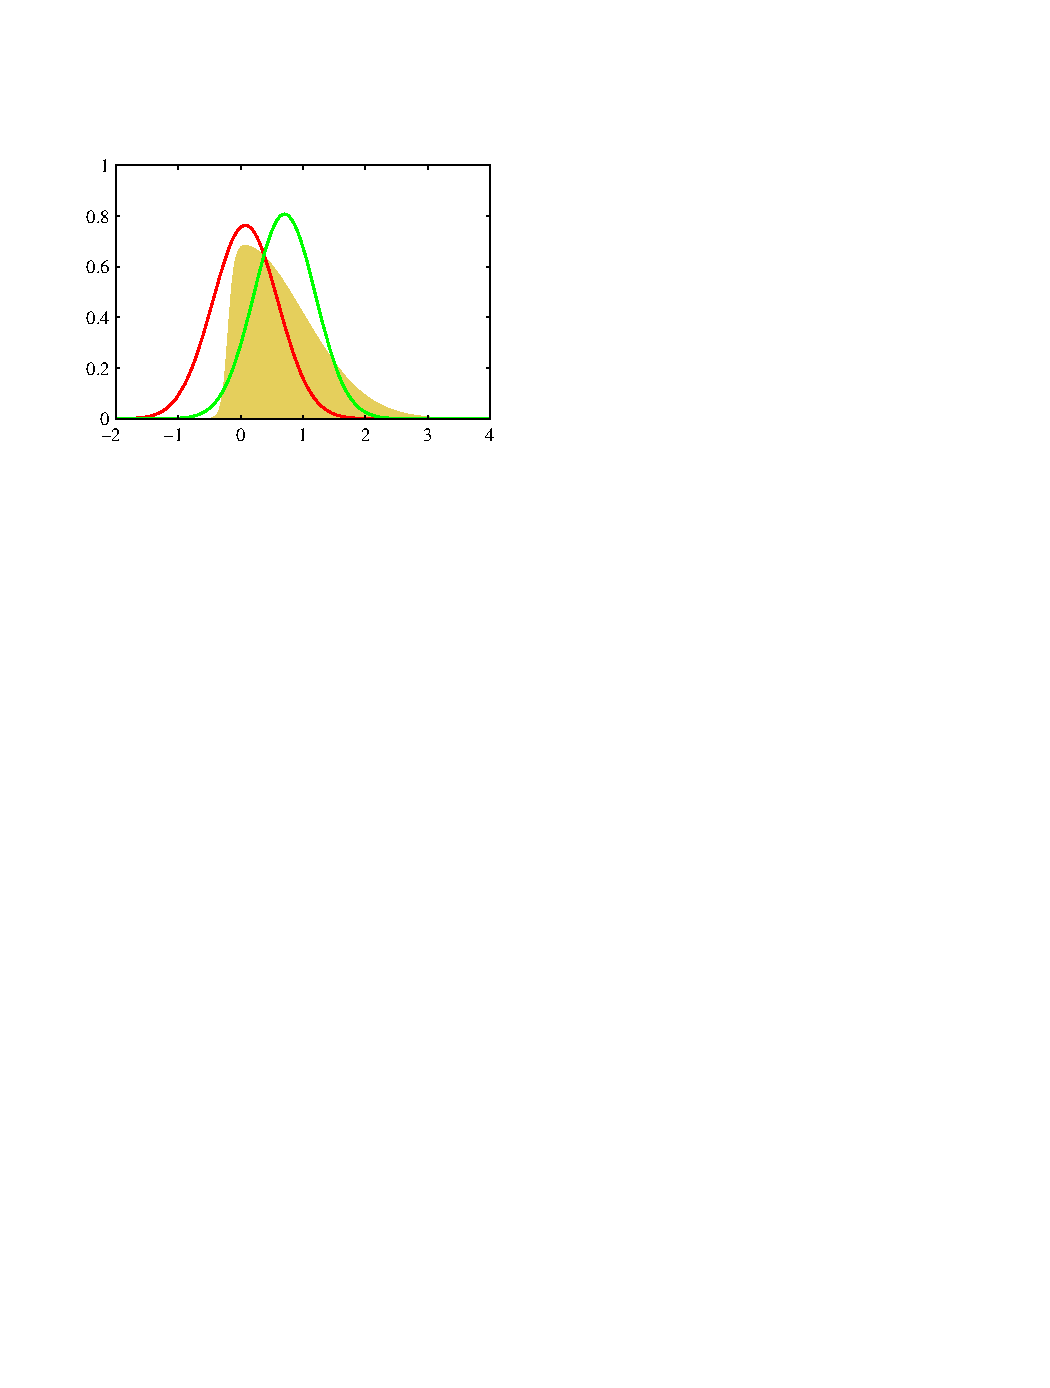
\includegraphics[width=0.4\textwidth]{img/bishop-fig-10-1.pdf}
\end{center}
\vspace*{-10pt}
\begin{itemize}
\item {\slshape solid yellow}: target; \ \ {\slshape red}: Laplace; \ \
  {\slshape green}: VB
\item \myemph{Laplace} located at posterior mode
\item \myemph{VB} located at approximate posterior mean
\end{itemize}
\vfill \hfill
{\footnotesize  --- Bishop (2006) {\slshape Pattern Recognition and Machine Learning}, fig.~10.1}


\sld{KL-Divergence Example}
%
\vspace*{-4pt}
\begin{center}
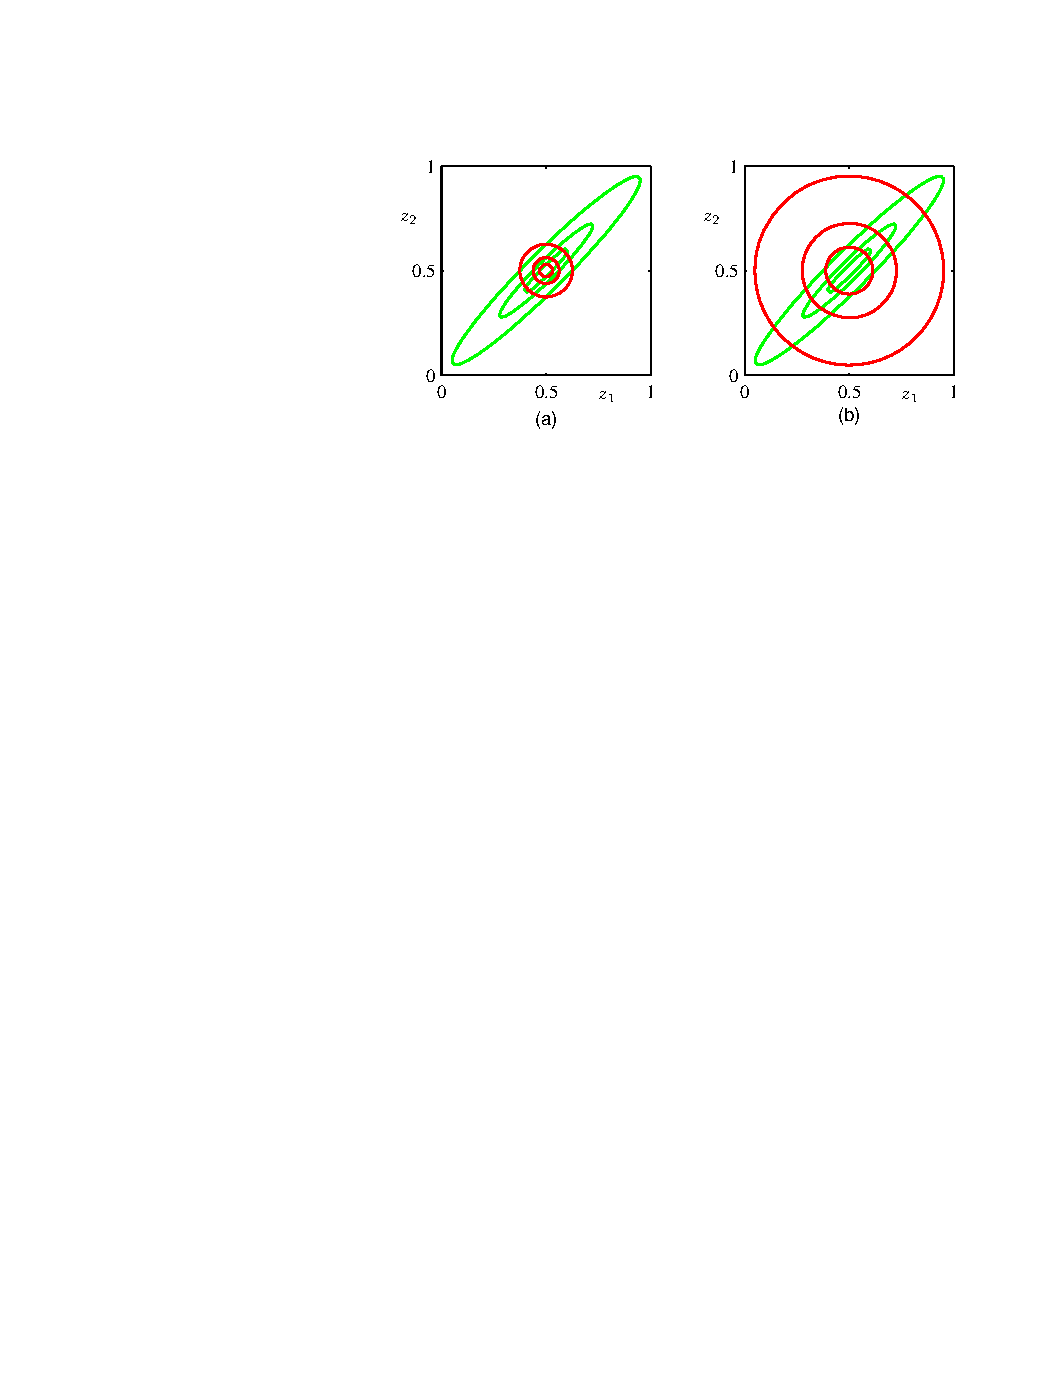
\includegraphics[width=0.5\textwidth]{img/bishop-fig-10-2.pdf}
\end{center}
\vspace*{-10pt}
\begin{subitemize}
\item \myemph{Green}: true distribution $p$; \ \ \myemph{Red}: best
  approximation $g$
\begin{subitemize}
\item[(a)] VB-like: $\mbox{KL}[g \, || \, p]$
\item[(b)] EP-like: $\mbox{KL}[p \, || \, g]$
\end{subitemize}
\item VB systematically \myemph{underestimates posterior variance}
\end{subitemize}
\vfill \hfill
{\footnotesize  --- Bishop (2006) {\slshape Pattern Recognition and Machine Learning}, fig.~10.2}


\sld{Stan's ``Black-Box'' VB}
%
\begin{itemize}
\item Traditional VB uses custom approximation $g()$ tailored to model
\begin{subitemize}
\item based on conjugacy and analytic updates
\end{subitemize}
\item Stan uses ``black-box VB'' with multivariate Gaussian $g$
\[
g(\theta|\phi) = \distro{MultiNormal}(\theta \, | \, \mu, \Sigma)
\]
for the \myemph{unconstrained posterior}
\begin{subitemize}
\item e.g., scales $\sigma$ log-transformed with Jacobian
\end{subitemize}
\item Stan provides two versions
\begin{subitemize}
\item Mean field: $\Sigma$ diagonal
\item General: $\Sigma$ dense
\end{subitemize}
\end{itemize}


\sld{Stan's VB: Computation}
%
\begin{itemize}
\item Use stochastic gradient descent optimization to optimize $\theta$
\item Requires gradient of KL-divergence w.r.t. $\theta$ up to constant
  \begin{subitemize}
  \item this requires nested Monte Carlo estimates
  \item requires reparameterization gradients for gradient descent
  \end{subitemize}
\item Approximate KL-divergence and gradient via Monte Carlo
\begin{subitemize}
\item only need approximate gradient calculation for soundness of L-BFGS
\item KL divergence is an expectation w.r.t. approximation $g(\theta|\phi)$
\item Monte Carlo draws i.i.d.\ from approximating multi-normal
\item derivatives with respect to true model log density via reverse-mode autodiff
\item so only a few Monte Carlo iterations are enough, though more much more stable if, e.g., in JAX
\end{subitemize}
\end{itemize}


\sld{Stan's VB: Computation (cont.)}
%
\begin{itemize}
\item To support compatible plug-in inference
\begin{subitemize}
\item draw Monte Carlo sample $\theta^{(1)}, \ldots, \theta^{(M)}$ with
\[
\theta^{(m)} \sim  \distro{MultiNormal}(\theta \, | \, \mu^{*}, \Sigma^{*})
\]
\item inverse transfrom from unconstrained to constrained scale
\item report to user in same way as MCMC draws
\vfill
\end{subitemize}
\item Future: reweight $\theta^{(m)}$ via importance sampling
\begin{subitemize}
\item with respect to true posterior
\item to improve expectation calculations
\end{subitemize}
\end{itemize}


\sld{Reverse-Mode Auto Diff}
%
\begin{itemize}
\item Eval gradient in (usually small) multiple of function eval time
\begin{subitemize}
\item independent of dimensionality
\item time proportional to number of expressions evaluated
\end{subitemize}
%
\item Result accurate to machine precision (cf. finite diffs)
\item Function evaluation builds up \myemph{expression tree}
\item Dynamic program propagates \myemph{chain rule} in reverse pass
\item Reverse mode computes $\nabla g$ in one
  pass for a function $f : \mathbb{R}^N \rightarrow \mathbb{R}$
\end{itemize}


\sld{Autodiff Expression Graph}
%
\\
\hspace*{6pt}
\begin{minipage}{0.5\textwidth}
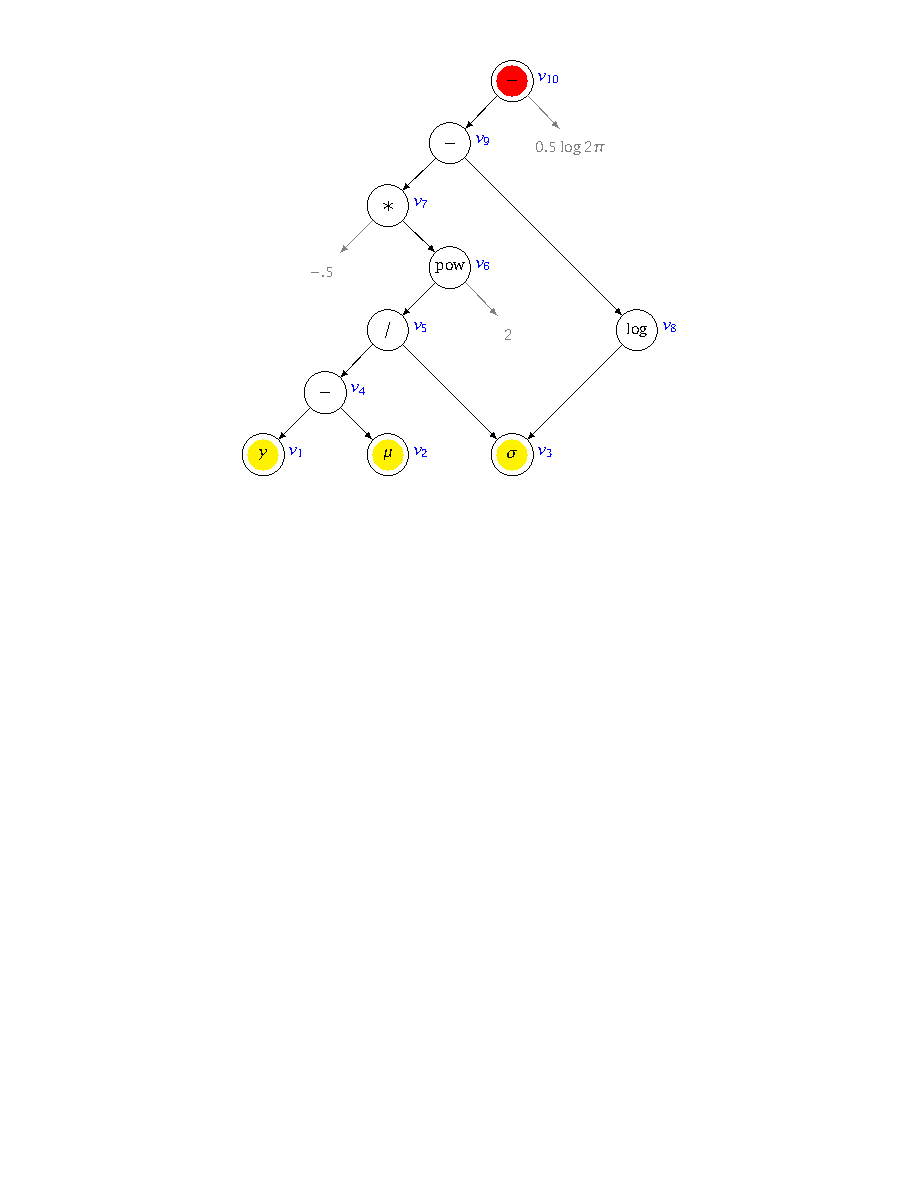
\includegraphics[width=\textwidth]{img/agrad-expression-graph.pdf}
\end{minipage}
\hspace*{-24pt}
\begin{minipage}{0.44\textwidth}
%
\footnotesize
\[
\begin{array}{l}
f(y, \mu, \sigma)
\\[4pt]
\mbox{ } \ = \ \log \left( \distro{Normal}(y|\mu,\sigma) \right)
\\[4pt]
\mbox{ } \ = \ -\frac{1}{2} \left( \frac{y - \mu}{\sigma} \right)^2
    - \log \sigma
    - \frac{1}{2} \log (2 \pi)
\end{array}
\]
\\
%
\[
\begin{array}{l}
\mbox{ } \hspace*{24pt}
\frac{\partial}{\partial y} f(y,\mu,\sigma)
\\[2pt]
\mbox{ } \hspace*{48pt} = \  -(y - \mu) \sigma^{-2}
\\[8pt]
\mbox{ } \hspace*{24pt} \frac{\partial}{\partial \mu} f(y,\mu,\sigma)
\\[2pt]
\mbox{ } \hspace*{48pt} = \ (y - \mu) \sigma^{-2}
\\[8pt]
\mbox{ } \hspace*{24pt} \frac{\partial}{\partial \sigma} f(y,\mu,\sigma)
\\[2pt]
\mbox{ } \hspace*{48pt} = \ (y - \mu)^2 \sigma^{-3} - \sigma^{-1}
\end{array}
\]
\end{minipage}


\sld{Autodiff Partials}
%
\begin{center}\footnotesize
\begin{tabular}{c||c|cc}
{\it var} & {\it value} & \multicolumn{2}{|c}{\it partials}
\\ \hline \hline
$v_1$ & $y$
\\[2pt]
$v_2$ & $\mu$
\\[2pt]
$v_3$ & $\sigma$
\\[2pt]
$v_4$ & $v_1 - v_2$ & $\partial v_4 / \partial v_1 = 1$
                   & $\partial v_4 / \partial v_2 = -1$
\\[4pt]
$v_5$ & $v_4 / v_3$ & $\partial v_5 / \partial v_4 = 1/v_3$
                    & $\partial v_5 / \partial v_3 = -v_4 v_3^{-2}$
\\[4pt]
$v_6$ & $\left(v_5\right)^2$
      & \multicolumn{2}{c}{$\partial v_6 / \partial v_5 = 2 v_5$}
\\[4pt]
$v_7$ & $(-0.5) v_6$ & \multicolumn{2}{c}{$\partial v_7 / \partial v_6
                                          = -0.5$}
\\[4pt]
$v_8$ & $\log v_3$ & \multicolumn{2}{c}{$\partial v_8 / \partial v_3 = 1/v_3$}
\\[4pt]
$v_9$ & $v_7 - v_8$ & $\partial v_9 / \partial v_7 = 1$
                    & $\partial v_9 / \partial v_8 = -1$
\\[4pt]
$v_{10}$ & $v_9 - (0.5 \log 2\pi)$
         & \multicolumn{2}{c}{$\partial v_{10} / \partial v_9 = 1$}
\end{tabular}
\end{center}

\sld{Autodiff: Reverse Pass}
%
{\small
\[
\begin{array}{rcl|l}
{\it var} & {\it operation} & {\it adjoint} & {\it result}
\\ \hline \hline
a_{1:9} & = & 0 & a_{1:9} = 0
\\
a_{10} & = & 1 & a_{10} = 1
\\ \hline
a_{9} & {+}{=} & a_{10} \times (1) & a_9 = 1
\\
a_{7} & {+}{=} & a_9 \times (1) & a_7 = 1
\\
a_{8} & {+}{=} & a_9 \times (-1) & a_8 = -1
\\
a_{3} & {+}{=} & a_8 \times (1 / v_3) & a_3 = -1 / v_3
\\
a_{6} & {+}{=} & a_7 \times (-0.5) & a_6 = -0.5
\\
a_{5} & {+}{=} & a_6 \times (2 v_5) & a_5 = -v_5
\\
a_{4} & {+}{=} & a_5 \times (1 / v_3) & a_4 = -v_5 / v_3
\\
a_{3} & {+}{=} & a_5 \times (-v_4 v_3^{-2}) & a_3 = -1 / v_3 + v_5 v_4 v_3^{-2}
\\
a_{1} & {+}{=} & a_4 \times (1) & a_1 = -v_5 / v_3
\\
a_{2} & {+}{=} & a_4 \times (-1) & a_2 = v_5 / v_3
\end{array}
\]
}


\sld{Stan's Reverse-Mode}
%
\begin{itemize}
\item Easily extensible \myemph{object-oriented} design
%
\item \myemph{Code nodes} in expression graph for primitive functions
\begin{subitemize}
\item requires \myemph{partial derivatives}
\item built-in flexible abstract base classes
\item \myemph{lazy evaluation} of chain rule saves memory
\end{subitemize}
%
\item Autodiff through templated C++ functions
\begin{subitemize}
\item templating on each argument avoids excess promotion
\end{subitemize}
%
\end{itemize}


\sld{Stan's Reverse-Mode (cont.)}
%
\begin{itemize}
\item Arena-based \myemph{memory management}
\begin{subitemize}
\item specialized C++ \code{operator~new} for reverse-mode variables
\item custom functions inherit memory management through base
\end{subitemize}
\item Nested application to support ODE solver
\end{itemize}


\sld{Stan's Autodiff vs.\ Alternatives}
%
\vspace*{-4pt}
\begin{itemize}
\item Stan is \myemph{fastest} (and uses least memory)
\begin{subitemize}
\item among open-source C++ alternatives
\end{subitemize}
\end{itemize}
\vspace*{-8pt}
\hfill \hfill
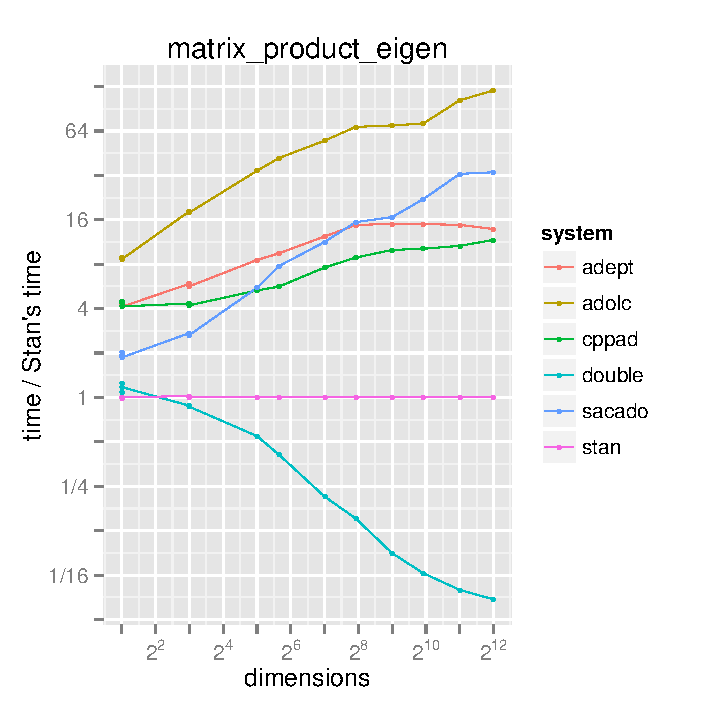
\includegraphics[width=0.4\textwidth]{img/autodiff-eval-matrix-product-eigen.pdf}
\hfill
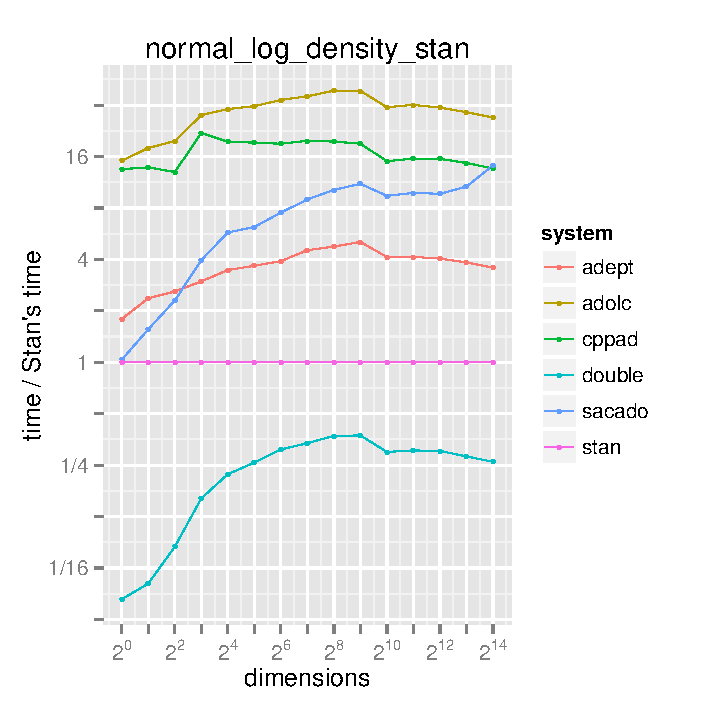
\includegraphics[width=0.4\textwidth]{img/autodiff-eval-normal-density.pdf}
\hfill \hfill


\sld{Forward-Mode Auto Diff}
%
\begin{itemize}
\item Evaluates expression graph forward from one independent variable
to any number of dependent variables
\item Function evaluation propagates \myemph{chain rule} forward
\item In one pass, computes $\frac{\partial}{\partial x} f(x)$
for a function $f : \mathbb{R} \rightarrow \mathbb{R}^N$
\begin{subitemize}
\item derivative of $N$ outputs with respect to a single input
\end{subitemize}
\end{itemize}


\sld{Stan's Forward Mode}
%
\begin{itemize}
\item Templated scalar type for value and tangent
\begin{subitemize}
\item allows higher-order derivatives
\end{subitemize}
\item Primitive functions propagate derivatives
\item No need to build expression graph in memory
\begin{subitemize}
\item much less memory intensive than reverse mode
\end{subitemize}
\item Autodiff through templated functions (as reverse mode)
\end{itemize}

\sld{Second-Order Derivatives}
%
\begin{itemize}
\item Compute Hessian (matrix of second-order partials)
\[
H_{i,j} = \frac{\partial^2}{\partial x_i \partial x_j} f(x)
\]
\item Required for Laplace covariance approximation (MLE)
\item Required for curvature (Riemannian HMC)
\item Nest reverse-mode in forward for \myemph{second order}
\item $N$ forward passes: takes gradient of derivative
\end{itemize}


\sld{Autodiff Functionals}
%
\begin{itemize}
\item Functionals map templated functors to derivatives
\begin{subitemize}
\item fully encapsulates and hides all autodiff types
\end{subitemize}
\item Autodiff functionals supported
  \begin{itemize}\small
  \item gradients: $\bigoh{1}$
  \item Jacobians: $\bigoh{N}$
  \item gradient-vector product (i.e., directional derivative): $\bigoh{1}$
  \item Hessian-vector product: $\bigoh{N}$
  \item Hessian: $\bigoh{N}$
  \item gradient of trace of matrix-Hessian product: $\bigoh{N^2}$
    \\ {\footnotesize (for SoftAbs RHMC)}
  \end{itemize}
\end{itemize}


\sld{Variable Transforms}
%
\begin{itemize}
\item Code HMC and optimization with $\mathbb{R}^n$ \myemph{support}
\item Transform constrained parameters to unconstrained
  \vspace*{-2pt}
  {\small
    \begin{itemize}
    \item lower (upper) bound: offset (negated) log transform
    \item lower and upper bound: scaled, offset logit transform
    \item simplex: centered, stick-breaking logit transform
    \item ordered: free first element, log transform offsets
    \item unit length: spherical coordinates
    \item covariance matrix: Cholesky factor positive diagonal
    \item correlation matrix: rows unit length via quadratic stick-breaking
    \end{itemize}
  }
\end{itemize}


\sld{Variable Transforms (cont.)}
%
\begin{itemize}
\item Inverse transform from unconstrained $\mathbb{R}^n$
\item Evaluate log probability in model block on natural scale
\item Optionally adjust log probability for change of variables
\begin{subitemize}
\item adjustment for MCMC and variational, not MLE
\item add log determinant of inverse transform Jacobian
\item automatically differentiable
\end{subitemize}
\end{itemize}

\sld{Parsing and Compilation}
%
\begin{itemize}
\item Stan's transpiler converts Stan code to a C++ class implementing the model and derivatives.
  \begin{subitemize}
  \item Originally C++ (Boost Spirit Qi), now OCaml (industry standard for parsing classes)
    \end{subitemize}
\item C++ model class \myemph{code generation} from AST
\item C++ code \myemph{compilation}
\item \myemph{Dynamic linking} for RStan, PyStan; static elsewhere
\end{itemize}


\sld{Coding Probability Functions}
%
\begin{itemize}
\item \myemph{Vectorized} to allow scalar or container arguments
  \\ {\footnotesize (containers all same shape; scalars broadcast as necessary)}
\item Avoid \myemph{repeated computations}, e.g. $\log \sigma$ in
  \hspace*{-18pt}
  {\small
    \begin{eqnarray*}
      \textstyle \log \, \mbox{\sf Normal}(y | \mu, \sigma)
      & = & \textstyle \sum_{n=1}^N \log \, \mbox{\sf Normal}(y_n | \mu,\sigma)
      \\[4pt]
      & = & \textstyle \sum_{n=1}^N  - \log \sqrt{2\pi} \ - \log \sigma \ -
      \frac{\textstyle y_n - \mu}{\textstyle 2\sigma^2}
    \end{eqnarray*}
  }
\item recursive \myemph{expression templates} to broadcast and cache scalars,
  generalize containers (arrays, matrices, vectors)
\item \myemph{traits} metaprogram to \myemph{drop constants} (e.g., $-\log
  \sqrt{2 \pi}$ or $\log \sigma$ if constant)
  and calculate intermediate and return types
\end{itemize}

\sld{BridgeStan}
\begin{itemize}
\item Provides interface to Stan models in Python, R, Julia, Rust, C, and C++.
  \begin{subitemize}
  \item variable transforms and inverse transforms for constraints (required for initialization on natural scale)
    \end{subitemize}
  \item evaluate of log density, gradients, Hessians (autodiff or finite diff of gradients where don't exist).
\item Allows algorithm testing using Stan models
  \begin{subitemize}
  \item not quite good enough for JAX normalizing flow evals
  \end{subitemize}
\end{itemize}



\end{document}